%!TeX root=../tese.tex
%("dica" para o editor de texto: este arquivo é parte de um documento maior)
% para saber mais: https://tex.stackexchange.com/q/78101/183146

% Apague as duas linhas abaixo (elas servem apenas para gerar um
% aviso no arquivo PDF quando não há nenhum dado a imprimir) e
% insira aqui o conteúdo dos capítulos do seu trabalho

%% ------------------------------------------------------------------------- %%
\chapter{Introduction}
\label{cap:introducao}

\begin{section}{Motivation}\label{sec:motivation}

The recent advances in both technological and computational fields induced an
increasingly faster expansion of software ecosystems. Developers create new
programs to supply the needs of the most diverse domains by coding new websites
in scripting languages, creating standalone desktop applications, adding new
functionalities to an operating system, and so on. Regardless of the reason
behind their development, it is true that their code will be, at some
point, transformed into machine language by a compiler or assembler, even if an
interpreter executes it.


%Os avanços nos campos tecnológicos e computacionais levaram uma enorme expansão
%Dos ecossistemas de \textit{software}. Novos programas são criados para
%Suprir as necessidades dos mais diversos domínios, seja através de sistemas web
%Codificados em linguagens de \textit{script}; ou por componentes para
%Sistemas operacionais destinados a embarcados, com a finalidade de controlar algum
%Recurso do \textit{hardware}. Independente da razão por trás do desenvolvimento
%Do \textit{software}, é certo que, em alguma etapa, seu código será transformado em linguagem de máquina por um compilador, mesmo que ele seja executado por um
%Interpretador.

A compiler is nothing more than a software that translates code from a
programming language $A$ into another language $B$ \citep{dragonbook}.  Compilers
are enormous programs, largely adopted by industry and academia, where a great
effort has been employed to produce efficient code -- but without any sacrifice
in correctness --. There are huge projects destined to develop and improve
them, such as the GNU Compiler Collections (GCC\footnote{https://gcc.gnu.org/})
and LLVM\footnote{https://llvm.org/}, capable of translating several languages
such as C, C++, and Fortran, to machine language. There are also smaller
projects such as F2C\footnote{https://www.netlib.org/f2c/}, a Fortran to C
compiler, used in systems where there is no Fortran compiler available. Such
compilers that translate from a high-level language into another high-level
language is often called a \textit{transpiler}.

%Um compilador nada mais é que um \textit{software} que traduz um código em uma linguagem
%de programação $A$ para outra linguagem $B$ \citep{dragonbook}.  Compiladores
%são programas enormes, largamente adotados pela indústria e academia, onde muito
%esforço e pesquisa foi e ainda é empregado para que eles produzam código
%eficiente, com destaque para a corretude. Existem projetos enormes destinados a desenvolvê-los e
%aprimorá-los, como o Gnu Compiler Collection
%(GCC\footnote{https://gcc.gnu.org/}), capaz de traduzir diversas linguagens
%como C, C++ e Fortran, para linguagem de máquina. Há também outros projetos
%menores como o F2C\footnote{https://www.netlib.org/f2c/}, um compilador de
%Fortran para C, utilizado em ambientes onde não há um compilador Fortran
%disponível.

Although it is possible to write code in machine language, which makes a compiler
unnecessary, it is extremely expensive and error-prone, apart from being an
uncommon practice in projects contemporary to this work \citep{githuboctoverse}
(see Figure \ref{fig:github_2017}). As an example, there is the Internal Revenue
Service (IRS) in the United States of America, which still maintains machines
compatible with the IBM System/360 due to the existence of several lines of
code written in assembly language for this architecture \citep{gao}.  This
problem earned media visibility after the  2018 Tax Day Failure
\citep{tax_failure}.

%Embora seja possível escrever código em linguagem de máquina, o que
%tornaria um compilador desnecessário, isto é extremamente caro e
%sujeito a erros, além de ser uma prática extremamente
%incomum nos projetos contemporâneos a este trabalho \citep{githuboctoverse} (vide
%Figura \ref{fig:github_2017}). Escrever programas em código de máquina tende a
%ser trabalhoso e financeiramente custoso, com difícil manutenção e quase impossível portabilidade.
%Um exemplo disso é o \textit{Internal Revenue Service} (IRS) dos Estados Unidos,
%que ainda mantém máquinas compatíveis com o IBM System/360 devido a existência no sistema
%de várias linhas de código escritas em linguagem de montagem para essa
%arquitetura \citep{gao}. Esse problema ganhou visibilidade na imprensa após a falha no
%\textit{Tax Day} de 2018 \citep{tax_failure}.

Compilers are used in projects of every size imaginable. Big projects can have
millions of lines of code, and even create new programming languages for an
easy way to develop new features. Therefore, the compilation process must be
fast, or else it may turn the project development unfeasible.  This means that
there are several studies employed to develop even faster algorithms for them,
beyond parallel computing techniques to improve the use the multicore processors,
increasingly common nowadays.

%Compiladores são usados em projetos dos mais variados tamanhos.
%Grandes projetos podem conter milhões de linhas de código, e até mesmo
%construir novas linguagens para facilitar o desenvolvimento de novas
%funcionalidades, e portanto o processo de compilação precisa ser rápido
%para viabilizar o seu desenvolvimento. Logo, muito estudo é aplicado
%para desenvolver algoritmos mais eficientes para eles, além de técnicas
%de computação paralela para aproveitar os recursos dos processadores
%\textit{multicore}, cada vez mais comuns.

%TODO: Deixar essa imagem mais legível
\begin{figure}[ht]
 \centering
 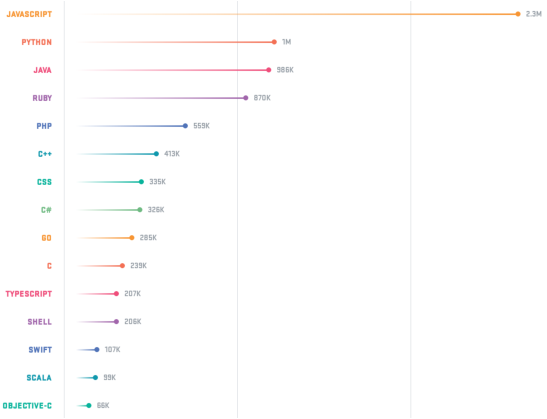
\includegraphics[scale=1.8]{github_2017.pdf}
 %\caption{As 15 linguagens mais usadas no GitHub em 2017. Fonte: \cite{githuboctoverse}}
 \caption{The 15 most used languages on GitHub in 2017. Source: \cite{githuboctoverse}}
 \label{fig:github_2017}
\end{figure}

\end{section}

\begin{section}{Parallelism in Compilation}

%O GCC é um compilador de código aberto amplamente usado tanto no meio
%acadêmico quanto na indústria. Por ser um grande projeto, o GCC contém uma
%linguagem própria para facilitar a adição de otimizações na geração de
%código, que em seguida é compilado em um único arquivo C, para (1)
%aproveitar as otimizações já implementadas no próprio compilador, e (2)
%evitar reescrever várias funcionalidades já implementadas. Infelizmente, este processo
%gera um gargalo na compilação do projeto em máquinas \textit{manycore}, pois o
%GCC não é capaz de compilar um arquivo em paralelo de maneira incremental.

%The GCC is a largely used Open Source compiler in both academic and industry
%environments. Being a large project, GCC has an additional language created to
%better express and facilitate optimizations in code generation, which is
%compiled into C++ to (1) reuse the optimizations already implemented in the
%compiler, and (2) avoid rewriting several functionalities already implemented.
%This process generates large files that must be compiled, causing a compilation
%bottleneck in the project because GCC is not capable of compiling a single file
%in parallel.

Currently, all parallelism in the compilation stage is provided either by the
GNU Make\footnote{https://www.gnu.org/software/make/}, which only provides a
per-file level granularity; or through the LTO infrastructure inside the compiler, which we
approach in Section \ref{chap:related_works}. The former, which we will label as
the \textit{classical compilation method}, may bottleneck the compilation in
manycore machines if there exists some file that dominates the compilation time.
The former may also have this bottleneck if the Whole Program Analysis (WPA) stage,
which runs serially, dominates the compilation time. While parallelizing
WPA is one way of tackling this problem, we have chosen to improve the parallelization
granularity on a single file compilation of \textit{classical compilation}.


%Atualmente, todo o paralelismo na fase de compilação é provido pelo GCC de
%duas maneiras distintas: ou pelo GNU Make\footnote{https://www.gnu.org/software/make/},
%que apenas fornece uma granularidade a nível dos arquivos; ou através da estrutura do
%LTO, que será abordada na Seção \ref{chap:related_works}. Esse gargalo pode parecer uma
%característica peculiar do projeto GCC, mas discussões com a comunidade levaram
%usuários a relatar o mesmo problema em seus projetos. Tal problema pode ser
%mitigado por um compilador que seja capaz de compilar um único arquivo em paralelo
%\citep{mailgcc}. Outra possível solução seria
%partir o arquivo em arquivos menores e utilizar o esquema de
%paralelismo já existente do GNU Make, mas isto implica em uma modificação na
%estrutura do projeto, o que pode não ser o ideal.

Since today the processors' manufacturers are increasing the power of their
products through parallelism over raw sequential power, compilers that can
profit from this resource could reduce the time taken when compiling a project
or even reduce execution time on script languages that rely on Just in Time
(JIT) compilation. It means a reduction in resource usage, such as
power, time, and thus money. So far, every parallelism found internally in
optimizing compilers was a consequence of a structure created to allow more
aggressive optimizations, such as the LTO \citep{glek2010optimizing}.

%Considerando que atualmente há uma tendência para que os processadores sejam
%cada vez mais paralelos, compiladores que usufruam deste recurso poderiam
%reduzir o tempo de compilação de um projeto, ou de uma suíte de testes que
%necessita recompilação antes de sua execução, economizando recursos no caso da
%computação ser cobrada por hora. Até então, o paralelismo empregado internamente
%em compiladores otimizadores foi consequência de uma estrutura criada para
%permitir otimizações mais agressivas e custosas, como o LTO
%\citep{glek2010optimizing}.

\end{section}

\begin{section}{Research Questions}\label{sec:rq}

%Deve ser observado que nem todos os processos de um compilador podem ser
%paralelizados. Compiladores operam em etapas que podem ser fortemente
%dependentes do resultado da etapa anterior. Por exemplo, ao compilar uma
%função em C, pode ser necessário saber se alguma outra foi declarada anteriormente; ou
%então o analisador sintático pode alterar um estado do analisador léxico para
%detectar variáveis de um novo tipo. Além disto, compiladores também se apoiam em algoritmos
%em grafos, cujo paralelismo é um desafio \citep{lumsdaine2007challenges}.

We must highlight that not every process inside a compiler can be parallelized.
Compilers that operate in steps can be strongly dependent on the resource
generated by some early pass.  For instance, when compiling a function in C, it
may be necessary to know if some function was declared early; or the syntactic
analyzer may change a state in the lexical analyzer to detect variables of a
new type. Not only that, but compilers also rely on graph algorithms, in
which parallelism is not trivial \citep{lumsdaine2007challenges}.

Therefore, this work is dedicated to the following research questions:

\begin{description}
    \item[\textit{RQ1}] - What is the main point of a compiler that can be improved with parallelism?
    \item[\textit{RQ2}] - What is the performance improvement after parallelizing a compiler?
	\item[\textit{RQ3}] - When compiling in parallel is faster than compiling sequentially?
	\item[\textit{RQ4}] - How does this impact the power consumption?
\end{description}

%Sendo assim, esse trabalho concentra-se em duas questões de pesquisas:
%\begin{description}
%    \item[\textit{QP1}] - Em que pontos um compilador pode usufruir de paralelismo?
%
%    \item[\textit{QP2}] - Qual é o ganho de desempenho ao paralelizar internamente um compilador?
%\end{description}

%essas questões de pesquisa visam propor uma alternativa ao LTO com foco
%em desenvolvimento incremental, e também cobrindo os casos onde o LTO produz binários menos
%eficientes através de melhorias no paralelismo do processo clássico de compilação.
%Para validar os resultados, este trabalho inclui a implementação no GCC de algumas das
%técnicas discutidas, além da utilização de técnicas de inferência estatística para
%análises no tempo total de compilação no projeto GCC e arquivos separados.

We present answers of these questions in the hope that they may be useful to software
developers so that they be aware of how compilers may impact the development
process of their projects, as well as compiler writers on how to improve
their software using parallelism. Thus, the main contribution of this work is
to provide ways to modify an industrial-scale compiler to
compile single files in parallel.

This work is divided into the following chapters: in Chapter
\ref{chap:fundamentacao}, we present some theoretical concepts regarding
Compiler Theory, the GCC,  and Parallel Computing to clarify some topics about this work.
Following that, Chapter \ref{chap:related_works} presents related work until
the state of art on this topic, with a brief discussion about their positive
and negative points. Then, Chapter \ref{chap:proposta} presents a general
version of the work, with an analysis of what needs to be improved,
contemplating the parallel architecture and the implementation planning, and presenting
our experiments about it later on Chapter \ref{cap:experiments}. Finally,
in Chapter \ref{chap:conclusions}, we present our conclusions about this work
and how it can be improved, with future works.

This work was supported by CAPES and Google Summer of Code (GSoC). For the
latter, we present our application plans in Appendix \ref{appendex1} for the threaded
parallelism project and Appendix \ref{appendix2} for the LTO parallelism project.  

%Este trabalho está dividido nos seguintes capítulos: no Capítulo
%\ref{chap:fundamentacao}, são apresentados conceitos teóricos como parte da
%Teoria de Compiladores e Computação Paralela para que seja possível
%compreender as questões acerca do trabalho.  Em sequência, o Capítulo
%\ref{chap:related_works} contém uma apresentação dos trabalhos relacionados
%a paralelismo de compiladores até o estado da
%arte nesse tópico, além de uma breve discussão sobre seus pontos positivos
%e negativos. Por fim, o Capítulo \ref{chap:proposta} apresenta uma visão geral
%do trabalho de fato, com uma análise de tempo consumido que permitiu
%identificar quais pontos necessitam de melhorias, além da
%proposta do trabalho, que contempla a arquitetura de paralelismo e o
%planejamento de sua implementação.

\end{section}

\chapter{Theoretical Background}
\label{chap:fundamentacao}

To avoid confusion regarding the various languages that the compiler works on,
we denote the following definitions on this work: Denote \textit{Source
Language}, as the language in which the code being compiled was originally
written; \textit{Intermediary Language} (IR) as the languages used internally in the
compiler; and \textit{Target Language} the language in which the compiler must
generate the code.

Compilers are large projects destined for the translation of source code
between distinct programming languages. Usually, compilers translate high-level
languages such as C, to assembly language, and those are the focus of our work.
We will not approach JIT compilers in this work, although they are very often
used in interpreted languages, such as Ruby or Python.

This chapter presents a brief introduction to the concepts used in this work.
In Section \ref{sec:parsing} we present a brief introduction about parsing
which are heavily used in a compiler. In Section \ref{sec:optimization} we
present all parts of the compiler pipeline to understand the compilation
phases. In Section \ref{sec:engineering} we discuss some software engineering
techniques that are employed when implementing compilers.  In Section
\ref{sec:gcc_compiler} we discuss the internals of the GCC compiler, from the
several Intermediate Representations of the compiler to the interaction between the parts.  In
\ref{sec:contributing} we present the details of the contributing process. In
Section \ref{sec:parallel_computing} we present some concepts from parallel
computing, which we use in this dissertation. And finally, Section
\ref{sec:power} briefly presents the concepts behind electrical power and energy
calculation, which we used in our experiments.

%Este capítulo apresenta uma breve introdução sobre os conceitos utilizados neste
%trabalho. Primeiro, são abordadas as partes do \textit{pipeline} de um compilador
%de maneira a entender os passos de compilação.
%Em seguida, discute-se como o compilador GCC apresenta esses tópicos implementados,
%além do seu uso no processo de compilação de um programa. Por fim, são
%apresentados alguns conceitos e algoritmos básicos sobre Computação Paralela.

%\begin{section}{Compiladores}

\begin{section}{Parsing}\label{sec:parsing}

Computer programs are written as a text file in some programming language,
which needs to be compiled or interpreted for execution. The first step of such
programs is to process the text file, validate the input with regard to the
language, and construct a data structure that is suitable for processing. This
process is named \textit{parsing}.

Parsing usually consists of two analysers: 
\begin{itemize}

\item \emph{Lexical Analysis}: responsible for reading a text file containing
the Source Code and splitting the words in the file into \textit{tokens}. As a
consequence, it is capable of applying some filters, \textit{e.g.} ignore commentaries,
identify numerical constants, remove unnecessary spaces, and replace a token
with another.  Lexical Analysers can also be used for macro expansion, as
implemented in the C preprocessor
(CPP)\footnote{https://gcc.gnu.org/onlinedocs/cppinternals/Lexer.html}.

Usually, Lexical Analysers are implemented using Deterministic Finite
Automatas, in which each acceptance state corresponds to a generated token.
This yields a fast, $O(n)$ algorithm for detecting tokens in the code, which
will be fed to the Lexical Analyser. There are even Lexical Analyser Generators
such as \textit{Flex}\footnote{https://www.gnu.org/software/flex/}, which are
extremely efficient.

\item \emph{Syntactic Analysis}: responsible to generate an Abstract Syntax
Tree (AST), inspecting the sequence of tokens provided by the Lexical Analyser,
or point out why the input string is invalid. The objective of a Syntatic
Analyser is to construct an AST by keeping track of the
reduction or derivation decisions with respect to the language grammar. The
decision of doing type analysis, checking for undefined usage of variables,
etc, can be done while building this AST, or postponed to a next stage, called
the Semantic Analysis.

Very often, these parsers are implemented either by emplying automatic
generated parsers such as \texttt{LALR}(1) algorithm provided by
\textit{Bison}\footnote{https://www.gnu.org/software/bison/}, or by
hand-implementing Recursive Descent parsers, which we present an example in
Figure \ref{fig:recursive-descent}. 

\end{itemize}

As an example of AST, Figure \ref{fig:ten-fact} illustrates a simple toy program in Java
that computes $10!$, and in Figure \ref{fig:ast-tenfact} we have a dump of its
AST.

\begin{figure}[ht]
      \begin{lstlisting}[
        language=pseudocode,
        style=pseudocode,
        style=wider,
        functions={},
        specialidentifiers={extern, call, public, static, class, void, String, int},
      ]
class Factorial {
    public static void main(String[] a) {
        System.out.println(new Fac().ComputeFac(10));
    }
}

class Fac {
    int teste;
    public int ComputeFac(int num) {
        int numxaux;
        int foo;
        if (num < 1)
            numxaux = 1;
        else
            numxaux = num * (this.ComputeFac(num-1));
        return numxaux;
    }
}
      \end{lstlisting}
	  \caption{Toy program to compute $10!$ in Java}
	  \label{fig:ten-fact}
\end{figure}


\begin{landscape}
\begin{figure}[ht]
    \begin{center}
     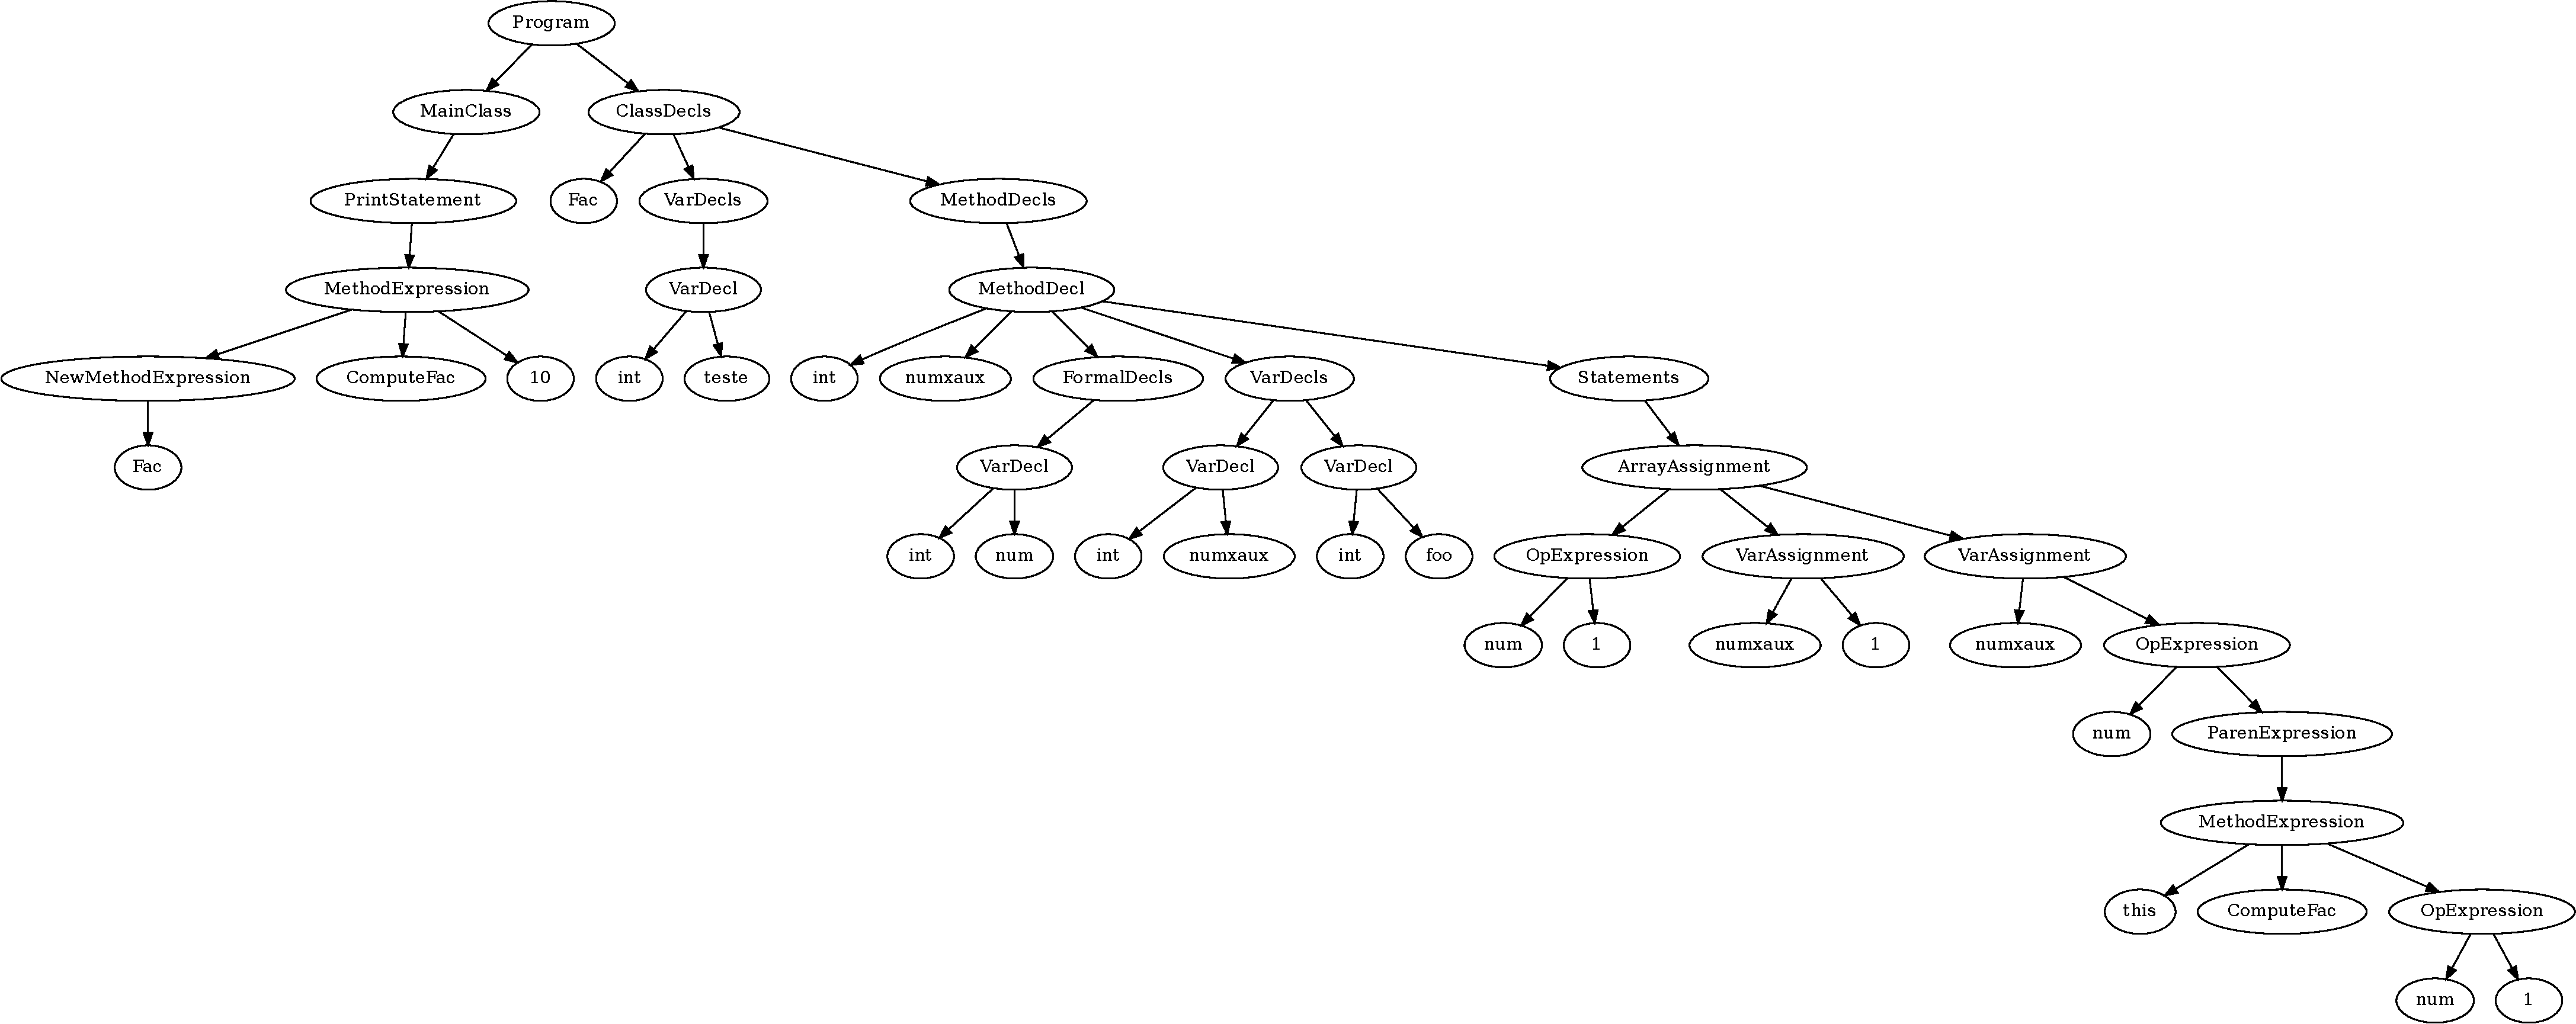
\includegraphics[width=0.8\paperheight]{ast.pdf}
	 \caption{Abstract Syntax Tree of Figure \ref{fig:ten-fact}}
	 \label{fig:ast-tenfact}
    \end{center}
\end{figure}
\end{landscape}

\end{section}

Another data structure constructed in this process is the Symbol Table.  The
Symbol Table, as the name suggests, is a table consisting of symbols
(variables, functions) with its declaration point, types, visibility, and other
information that the compiler writer might find useful. It is very often
constructed in this parsing process as the Syntactic Analyser detects variables
and functions, which may be used later to perform type checks and references to
undefined symbols. Figure \ref{fig:lexico_sintatico} illustrates how these
three pieces communicate with each other.

\begin{figure}
\tikzstyle{block} = [rectangle, draw, fill=white,
    text width=6em, text centered, rounded corners, node distance=9cm, auto, minimum height=2em]
\tikzstyle{line} = [draw, -latex]
\tikzstyle{cloud} = [draw, ellipse,fill=white, node distance=2cm,
    minimum height=2em]

%TODO: Adcionar a tabela de símbolos aqui.
\begin{center}
\scalebox{0.8}{
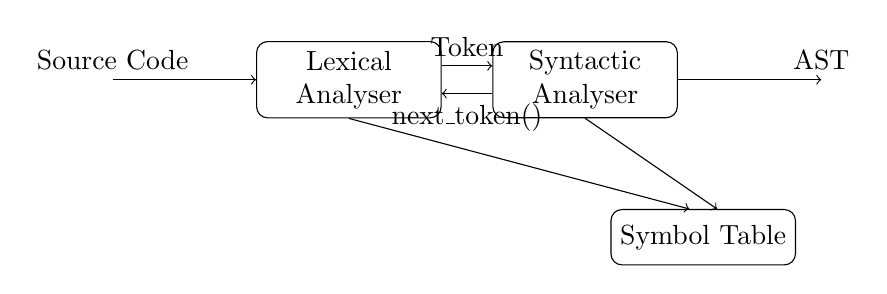
\begin{tikzpicture}[node distance = 3cm, auto]
    % Place nodes
    \node [block]                    (lexico) {Lexical Analyser};
    \node [block, right of = lexico] (sintatico) {Syntactic Analyser};
    \node [block] at (4.5, -2) (symtab) {Symbol Table};
    \coordinate [left of=lexico]     (fonte);
    \coordinate [right of=sintatico] (ast);

    % Draw edges
    \draw[->]    ([yshift=0.5em] lexico.east)       -- ([yshift=0.5em] sintatico.west) node[midway] {Token};
    \draw[->]    ([yshift=-0.5em] sintatico.west)   -- ([yshift=-0.5em] lexico.east)    node[midway] {next\_token()};
    \draw[->]    (fonte.west)                       -- (lexico.west)    node[pos=0, above] {Source Code};
    \draw[->]    (sintatico.east)                   -- (ast.west)   node[pos=1, above] {AST};
	\draw[->]    (sintatico.south)                  -- ([xshift=0.5em]symtab.north);
	\draw[->]    (lexico.south)                     -- ([xshift=-0.5em]symtab.north);

\end{tikzpicture}
}
\end{center}

\caption{Interactions between the Lexical, Syntactic Analyser and the Symbol Table}
\label{fig:lexico_sintatico}
\end{figure}

More details about how to construct parsers, what is a grammar in the context
of programming languages, and an brief introduction to parsing theory can be
seen in Appendix \ref{sec:apendix-parser}.


\begin{section}{Compiler Optimization}\label{sec:optimization}

Today industrial compilers are what we call to be an ``Optimizer Compiler'', because
it not only do a direct translation to another language, but because it
tries to generate faster code than the input code created by the programmer
while still maintaining its correctness.

There are several data structures and frameworks which is often used to
develop optimizations, which we briefly present here.

%Given a program, there are two disjoint set of optimizations in which we
%operate on:
%\begin{itemize}
%	\item \textit{Architecture-free Optimizations}: Any optimization that
%	does not require any interaction with anything specific about the target
%	machine in which the code is being compiled to. Example: \textit{constant
%	propagation}.
%
%
%	\item \textit{Architecture-dependent Optimizations}: Any optimization that
%	require interaction with something specific about the target machine in
%	which the code is being compiled to. Example: \textit{register allocation}.
%\end{itemize}
%
%Furthermore, we can also separate the set of all optimizations is two
%others disjoint sets:
%
%\begin{itemize}
%	\item \textit{Intraprocedural Optimizations}: Optimizations which only uses
%	information inside the function. Example: \textit{register allocation}.
%
%	\item \textit{Interprocedural Optimizations}: Any optimization that
%	require interaction with something specific about the target machine in
%	which the code is being compiled to. Example: \textit{function inlining}.
%\end{itemize}
%
%This last one is very interesting in the point of parallelization. Intraprocedural
%Optimizations can be run in parallel per function, as there is no dependency between
%two functions. Interprocedural, by the other hand, has no clear parallelization point.

\begin{subsection}{Three-Address Code Form}

One issue with large expressions is that it is very hard to find common
subexpressions and eliminate them. For instance, consider the mathematical
expression:
$$y = x \times x + x \times x $$
this expression can be simplified to $y = 2x^2$, but how
can a compiler know this? One could break this expression in the following
sequence of statements:
\begin{align}
t_1 &= x \times x \nonumber \\
t_2 &= x \times x \nonumber \\
y &= t_1 + t_2 \nonumber
\end{align}
now, some information is evident here. First is that $t_2 = t_1$,
and therefore $t_2$ is a completely unnecessary variable, and can be
eliminated from the program, which will lead to $y = t_1 + t_1$, which is
evident that can be simplified further to $y = 2 \times t_1$, which will lead
to the sequence of statements:

\begin{align}
t_1 &= x \times x \nonumber \\
y &= 2 \times t_1 \nonumber
\end{align}
which satisfy the following definition:
\begin{definition}
	A program is in Three-Address Code (3AC) format if every expression is
	in $c = a \texttt{<op>} b$ form, where $a, b, c$ are variables or
	literal constants.
\end{definition}

Not only used to detect common subexpressions, the 3AC representation is also
useful when allocating registers to variables, once instructions usually only
take two operands as argument (for instance, the \texttt{add} instruction in
x86). 

\end{subsection}

\begin{subsection}{Control-Flow Graph}

Programs consist of more than a linear sequence of statements, as there are
jumps, loops, and gotos, which we call \textit{flow-divergence}. Those
divergences can be modeled through a \textit{Control-Flow Graph}, which
illustrates jumps explicitly.

For example, consider the program in Figure \ref{fig:1-norm_program}.  Here,
the first two statements $i \leftarrow 0$ and $\textit{sum} \leftarrow 0$ are
always executed in the sequence, so there is no need to explicitly show any
kind of jump between these two statements. However, the \texttt{if} and
\texttt{else} will result in a \textit{flow-divergence} depending on the value
of \texttt{x[i]}, which is illustrated in Figure \ref{fig:1-norm_program:cfg}. 
\begin{figure}[ht]
\centering
  \begin{subfigure}[b]{0.40\textwidth}
      \begin{lstlisting}[
        language=pseudocode,
        style=pseudocode,
        style=wider,
        functions={},
        specialidentifiers={extern, call},
      ]
        function norm_1(x[n])
            sum := 0
			i := 0
            while (i < n) {
                if (x[i] < 0)
                    sum -= x[i]
                else
                    sum += x[i]
				i := i + 1
            }
            return sum
        end
      \end{lstlisting}
	  \caption{Program that computes the 1-norm of a vector}
	  \label{fig:1-norm_program}
  \end{subfigure}
  \begin{subfigure}[b]{0.40\textwidth}
    \tikzstyle{line} = [draw, -latex]
    \tikzstyle{node} = [draw, rectangle]
    \begin{center}
    \scalebox{0.5}{
    \begin{tikzpicture}[node distance = 2.3cm, minimum height = 1cm, auto]
        % Place nodes
        \node [node]                    (source) {$s_0$};
        \node [node, below of = source] (head) {while};
        \node [node, below of = head]   (check) {if};
        \coordinate[below of = check]            (c2);
        \node [node, left of = c2]  (true) {true};
        \node [node, right of = c2]   (false) {false};
        \node [node, below of = c2]   (merge) {$i \leftarrow i + 1$};
        \node [node, left of = head]   (return) {return};
        \coordinate[right of=false]    (c3);

        % Draw edges
        \draw[->]    (source)         -- (head);
        \draw[->]    (head)           -- (check);
        \draw[->]    (check)          -- (true);
        \draw[->]    (check)          -- (false);
        \draw[->]    (true)       -- (merge);
        \draw[->]    (false)      --  (merge);
        \draw    (merge.east) to [out=0, in=-90]  (c3);
        \draw[->]    (c3) to [out=90, in=0]  (head);

        \draw[->]    (head.west)  to [out=180, in=180] (return.east);
    \end{tikzpicture}
    }
    \end{center}
  \caption{Control-Flow Graph of the Program}
  \label{fig:1-norm_program:cfg}
  \end{subfigure}
\end{figure}
It is useful to model when those flow-divergences jumps will occur, which
motivates the definition of a \textit{basic-block}.

\begin{definition}
A \textbf{basic-block} is the maximum sequence of statements in which there is
no flow-divergence.
\end{definition}

For instance, both statements $i \leftarrow 0$ and $\textit{sum} \leftarrow 0$ belongs
to the same basic-block, as there are no \textit{flow-divergence} between
those two statements. However, \texttt{if (x[i] < 0)} and \texttt{sum += x[i]}
belongs to distinct basic-blocks. Figure \ref{fig:1-norm_program:cfg} shows
the basic block for the program. The definition of a Control-Flow Graph is
as follows.

\begin{definition}
	A Control-Flow Graph (CFGraph) $G = (V, E, s_0, F)$ is a directed-graph,
	where each $v \in V$ is a basic-block containing a list of statements,
	an edge $(u, v) \in E \ssq V \times V$ if the flow can jump from
	$u$ to $v$, $s_0 \in V$ is the source node, in which the execution
	starts, and $F \ssq V$ is the set of end blocks, in which there
	are no outgoing edges to other nodes.
\end{definition}

Control-Flow Graphs have several usages in compilers and static analyzers. For
instance, the analyzer can detect loops in codes that do not use any
conventional loop operands such as \texttt{while} or \texttt{for} (e.g. the
code has several \texttt{goto}s), and even detect unreachable code by verifying
if a certain node is reachable from the CFGraph source node. But its main usage
is on dataflow frameworks, which we will introduce in Subsection \ref{sec:dataflow}.

\end{subsection}

\begin{subsection}{Posets and Lattices}

One of the mathematical theories to model \textit{order between binary
relations} is called \textit{Lattice Theory}. One clear example of order in
mathematics is the set of all integers $\mathbb{Z}$ with the binary, partial
order relation $\leq$. However, when the set in which we are working on is
abstract, for instance which variables are live on some program point, such order relation turns out to be convoluted. Nevertheless, finding
such order in these abstract structures may be helpful.

\begin{definition}
A Partial Order $\sqsq$ over a set $S$ is a binary relation that is:
\begin{itemize}
	\item Reflexive: For all $s \in S$, $s \sqsq s$.
	\item Transitive: For all $q, r, s \in S$, if $q \sqsq r$ and $r \sqsq s$, then
	$q \sqsq s$.
	\item Anti-Symmetric: For all $r, s \in S$, if $r \sqsq s$ and $s \sqsq r$,
	then $r = s$.

A partially ordered set (poset) denoted by $\mathcal{P} = (S, \sqsq)$, is a
set $S$ with a partial order $\sqsq$. Furthermore, we say that $x \in \mathcal{P}$
if and only if $x \in S$.
\end{itemize}
\end{definition}

We can also define an operation on posets based on order, which is useful if
it denotes the amount of information we currently have so far.

\begin{definition}
Let $\mathcal{P} = (L, \sqsq)$ be a poset. A subset $S \ssq L$ has an
\textit{upper-bound} $l \in L$ if for every $r \in S$, then $r \sqsq l$.
Furthermore, $l$ is the \textit{least upper-bound} if for every other
upper-bound $x \in L$ of $S$, $r \sqsq x$.
\end{definition}

\begin{definition}
Let $\mathcal{P} = (L, \sqsq)$ be a poset. A subset $S \ssq L$ has an
\textit{lower-bound} $l \in L$ if for every $r \in S$, then $l \sqsq r$.
Furthermore, $l$ is the \textit{greatest lower-bound} if for every other
lower-bound $x \in L$ of $S$, $x \sqsq r$.
\end{definition}

\begin{definition}
The binary \textit{join} operator, denoted as $l \sqcup r$, is the
least upper-bound of the subset $\{r, s\}$ of a poset $\mathcal{P}$.
\end{definition}

\begin{definition}
The binary \textit{meet} operator, denoted as $l \sqcap r$, is the
greatest upper-bound of $\{r, s\}$ of a poset $\mathcal{P}$.
\end{definition}

One can clearly see that both $\sqcup$ and $\sqcap$ satisfies the
following three properties:

\begin{itemize}
	\item Idempotence: For all $r \in S$: $r \sqcup r = r$, and $r \sqcap r = r$ 
	\item Commutativity: For all $r, l \in S$: $l \sqcup r = r \sqcup l$, and
	$l \sqcap r = r \sqcap l$
	\item Associativity: For all $l, r, s \in S$: $(l \sqcap y) \sqcap s = l \sqcap (r \sqcap s)$
\end{itemize}

%Now, a desired condition to have in a poset is the \textit{ascending chain} (or
%\textit{descending chain}, according to the analysis) condition, so that we know
%that we know that eventually the propagation in the graph stabilizes.
%
%\begin{definition}
%A totally ordered chain $S = {s_1, s_2, \cdots}$ of a poset $\mathcal P$ is a
%\textit{ascending chain} if given two integers $1 \leq i \leq j$, then
%$s_i \sqsq s_j$. Analogously, $S$ is a \textit{descending chain} if
%$x_j \sqsq x_i$.
%\end{definition}

Notice that for a poset, the result of both $\sqcup$ and $\sqcap$ is not
required to be in the poset (\textit{i.e.} the operation is not closed).
That is the main difference between a poset and a \textit{lattice}.
If $\sqcap$ is closed, we have a \textit{meet semi-lattice}.

\begin{definition}
	A poset $\mathcal{P} = (L, \sqsq)$ is a \textbf{meet semi-lattice} if
	for every non-empty subset $S \ssq L$, $\left(\bigsqcap_{s \in S} s \right) \in L$.
\end{definition}

There is also structures which satisfies stronger claims, which is the case
of \textit{lattices} and \textit{complete lattices}.

\begin{definition}
	A poset $\mathcal{P} = (L, \sqsq)$ is a \textbf{lattice} if for every
	non-empty finite subset $S \ssq L$, both $\left(\bigsqcup_{s \in S} s\right) \in L$
	and $\bigsqcap_{s \in S} s \in L$.
\end{definition}

\begin{definition}
	A poset $\mathcal{P} = (L, \sqsq)$ is a \textbf{complete lattice} if
	for every subset $S \ssq L$, both $\left( \bigsqcup_{s \in S} s \right) \in L$
	and $\left(\bigsqcap_{s \in S} s \right) \in L$.
\end{definition}

It is also useful to denote the greatest and the smallest element of a lattice.

\begin{definition}
	The \textbf{top} element of a lattice $\mathcal{L}$ is $\top = \bigsqcup_{l \in \mathcal{L}} l$. Similarly, the \textbf{bottom} element is $\bot = \bigsqcap_{l \in \mathcal{L}} l$.
\end{definition}

However, for dataflow frameworks, it is not required to work on a complete
lattice. A meet semi-lattice is enough.

We can also define functions over a lattice in a similar way that functions can
be defined in $\mathbb{Z}$. From all functions that could be defined over a
lattice, we are interested in monotone functions, which helps to ensure that
some analysis ends after a finite number of iterations.

\begin{definition}
	A function $f:\mathcal{L} \longrightarrow \mathcal{L}$ is monotonic if and only if
	for $x, y \in \mathcal{L}$:
	$$x \sqsq y \Rightarrow f(x) \sqsq f(y)$$.
\end{definition}

Lattices have an important role in the formal definition of dataflow
frameworks, as they are often used to prove that the analysis always halts with
some result for every input program.
For instance, the fact that the meet operation always gives a result closer to
the bottom element guarantees that frameworks using a meet semilattice will
always converge to a result.

\end{subsection}

\begin{subsection}{Dataflow Analysis}\label{sec:dataflow}

Dataflow Analysis is a technique to collect and propagate information across a
Control-Flow Graph. It is used not only in compilers but also in static code
analysis in general in the field of Software Engineering.

When analyzing a program's function, it is useful to know at a certain point,
what properties do hold to decide for an optimization.  Incorrectly guessing
some property may result in an incorrect transformation. Therefore, it is
useful to employ a way to propagate information across the Control-Flow Graph
of a function. This is where Dataflow Analysis is useful.

Given a Control-Flow Graph $G = (V, E, s_0, F)$ of a program, construct a
complete or meet lattice $\mathcal{L}$, which represents a set of possible
information that is true in a certain point of a program.  Then, we define a
set of \textit{flow functions} $\mathcal{F}_G = \{f_1, f_2, \cdots, f_{|V|}\}$,
where $f_v: \mathcal{L} \longrightarrow \mathcal{L}$, for each node $v \in V$.
These functions will generate, destroy, or transform information contained in
each vertex of the graph. These functions must be of the form of
\textit{forward analysis}, which yields Equation \ref{eq:forward}, or
\textit{backward analysis}, which yields Equation \ref{eq:backward}.

\begin{equation}\label{eq:forward}
	\texttt{in[} v \texttt{]} = \begin{cases}
	  BI,& \text{if } v = s_0 \\
	  \bigsqcap_{p \in \text{pred}(v)}f_p(\texttt{in[}p\texttt{]}) ,& \text{otherwise} \\
	\end{cases}
\end{equation}

\begin{equation}\label{eq:backward}
	\texttt{out[} v \texttt{]} = \begin{cases}
	  BI,& \text{if } v \in F \\
	  \bigsqcap_{p \in \text{succ}(v)}f_p(\texttt{out[}p\texttt{]}) ,& \text{otherwise} \\
	\end{cases}
\end{equation}

Equations \ref{eq:forward} and \ref{eq:backward} can be solved by
\textit{propagation}, just applying the equation to each vertex until there is
no more new information being generated or destroyed (in other 	words, the
equation \textit{converges}). Some tricks can be employed for a faster
convergence, \textit{e.g.}, start propagation from $s_0$ in forward analysis,
and from any $v \in F$ in the backward analysis.  Algorithms for solving those
equations in a general way can be found in \citep{khedker2009data}.

Figure \ref{fig:functions_dataflow} illustrates how each function of
$\mathcal{F}_G$ are related to each node of the $G$. Furthermore, Figure
\ref{fig:meet_dataflow} illustrates how the meet operator $\bigsqcap$ is used
to combine the information generated by the predecessors and send it to the
successors of a node, for the \textit{forward analysis} case.

\begin{figure}[ht]
\centering
  \begin{subfigure}[b]{0.40\textwidth}
	 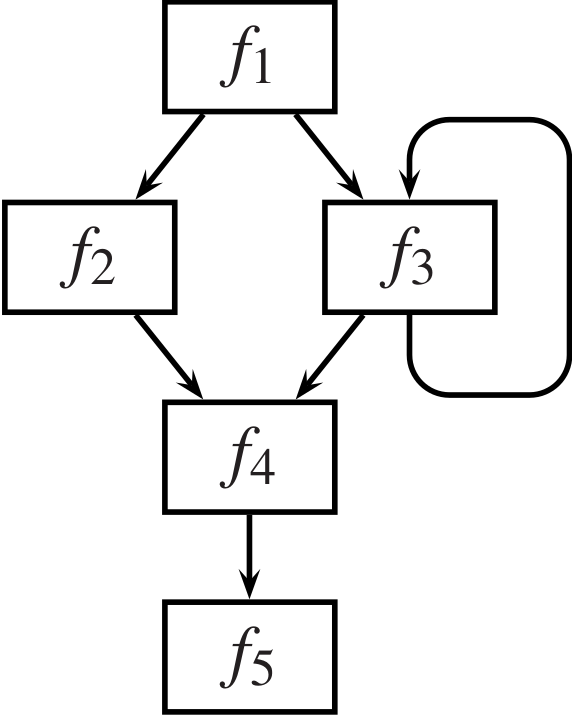
\includegraphics[scale=0.2]{functions_dataflow.png}
	  \caption{Dataflow Flow Functions. One for \\ each vertice of $G$. \citep{khedker2009data}}
	  \label{fig:functions_dataflow}
  \end{subfigure}
  \begin{subfigure}[b]{0.40\textwidth}
	 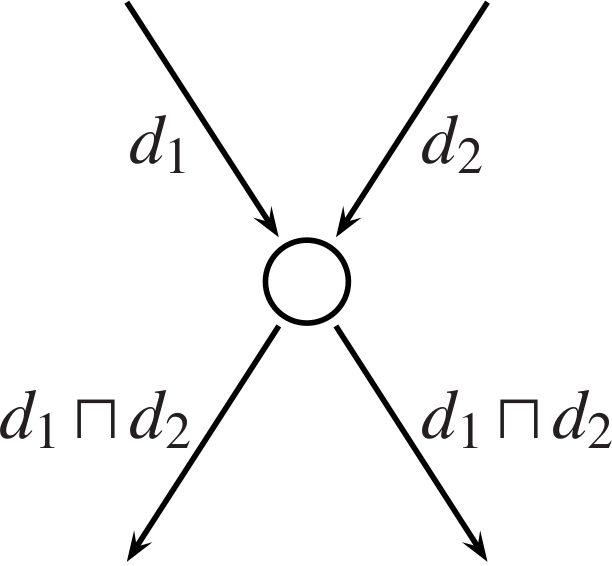
\includegraphics[scale=0.2]{meet_dataflow.png}
	  \caption{Meet operation on a vertice, combining the generated information. \citep{khedker2009data}}
	  \label{fig:meet_dataflow}
  \end{subfigure}
  \label{fig:dataflow}
\end{figure}

	Therefore, in an abstract way, we can define a dataflow framework instance as
	\begin{definition}
		An instance of dataflow framework is a 4-uple $(G, \mathcal{L}, \bigsqcap, \mathcal{F}_G)$,
		where
		\begin{itemize}
			\item $G = (V, E, s_0, F)$ is a Control-Flow Graph.
			\item $\mathcal{L}$ is a meet semi-lattice satisfying the descending chain condition.
			\item $\bigsqcap$ is the meet operator of $\mathcal{L}$.
			\item $\mathcal{F}_G = \{f_1, f_2, \cdots, f_{|V|}\}$ is the set of monotonic transfer
			functions, one for each node $v \in V$, of the form of Equation \ref{eq:forward} or \ref{eq:backward}.
		\end{itemize}
	\end{definition}

Dataflow frameworks have an important role in compilers and software static
analysis, as they are often used to model problems that require information to
be propagated through the CFGraph. Several problems can be solved by finding a
solution to a dataflow equation, such as constant folding, liveness analysis,
pointer alias, and so on. We will present liveness analysis as an example, once
it is used in the register allocation phase.

\begin{subsubsection}{Liveness Analysis}

One example of a problem that can be solved with dataflow analysis is the
\textit{liveness analysis}.
The purpose of it is to find, given a point in a CFGraph, if a certain variable
will be used in the future. This step is important to the register allocation
phase because if a certain variable is used in the future, we may need to keep
its value in a register for future use. If the variable is not live anymore,
then we can use that register to hold another variable, thus improving register
usage in the final code.  \cite{khedker2009data} defines the liveness
analysis formally as:

\begin{definition}

Let $G = (V, E, s_0, F)$ be a CFGraph and $\mathbb{V}$ be the set of all
variables of $G$. A variable $x \in \mathbb{V}$ is \textbf{live} at a program
point $v \in V$ if there exists a path from $v$ to $w \in F$ which contains a
use of $x$ which is not preceeded by its definition.
\end{definition}

Therefore, a CFGraph $G$, a dataflow framework instance for this would be:
$(G, \mathcal{L}, \bigsqcap, \mathcal{F}_G)$, where
\begin{itemize}
	\item $\mathcal{L} = (2^\mathbb{V}, \supseteq)$, where $\mathbb{V}$ is the set of variables in the function represented by $G$.
	\item $\bigsqcap$ is the union operator $\bigcup$.
	\item $F_G = \conj{\texttt{in[} v \texttt{]}}{v \in V}$ where
	$\texttt{in[} v \texttt{]} = (\texttt{out[} v \texttt{]} - \texttt{kill[} v \texttt{]}) \cup \texttt{gen[} v \texttt{]}$.
\end{itemize}
which yields the dataflow equation:
\begin{equation}\label{eq:liveness}
\begin{split}
	\texttt{in[} v \texttt{]} &= (\texttt{out[} v \texttt{]} - \texttt{kill[} v \texttt{]}) \cup \texttt{gen[} v \texttt{]} \\
	\texttt{out[} v \texttt{]} &= 
	\begin{cases}
	  \emptyset,& \text{if } v \in F \\
	  \bigcup_{p \in \text{succ}(v)}\texttt{in[}p\texttt{]} ,& \text{otherwise} \\
	\end{cases}
\end{split}
\end{equation}

In this equation, $\texttt{gen[} v \texttt{]}$ represents the variables which
turns to be live at vertex $v$, and $\texttt{kill[} v \texttt{]}$ are the
variables which liveness are no longer valid at vertex $v$. For instance,
consider the CFGraph in Figure \ref{fig:cfg_liveness}. Here, we work on the set
$\mathbb{V} = \{a, b, c, d\}$.  We present the solution of Equation
\ref{eq:liveness} is presented in Table \ref{fig:table_cfg} using the
propagation technique. There, for instance, we can see that $d$ is not used
anywhere in the program because $d \not\in \ttt{out[}n_1\ttt{]}$. This means
that the variable $d$ can be discarded from the program, and therefore no
register or memory space is necessary to hold this variable.

\begin{figure}
\centering
	 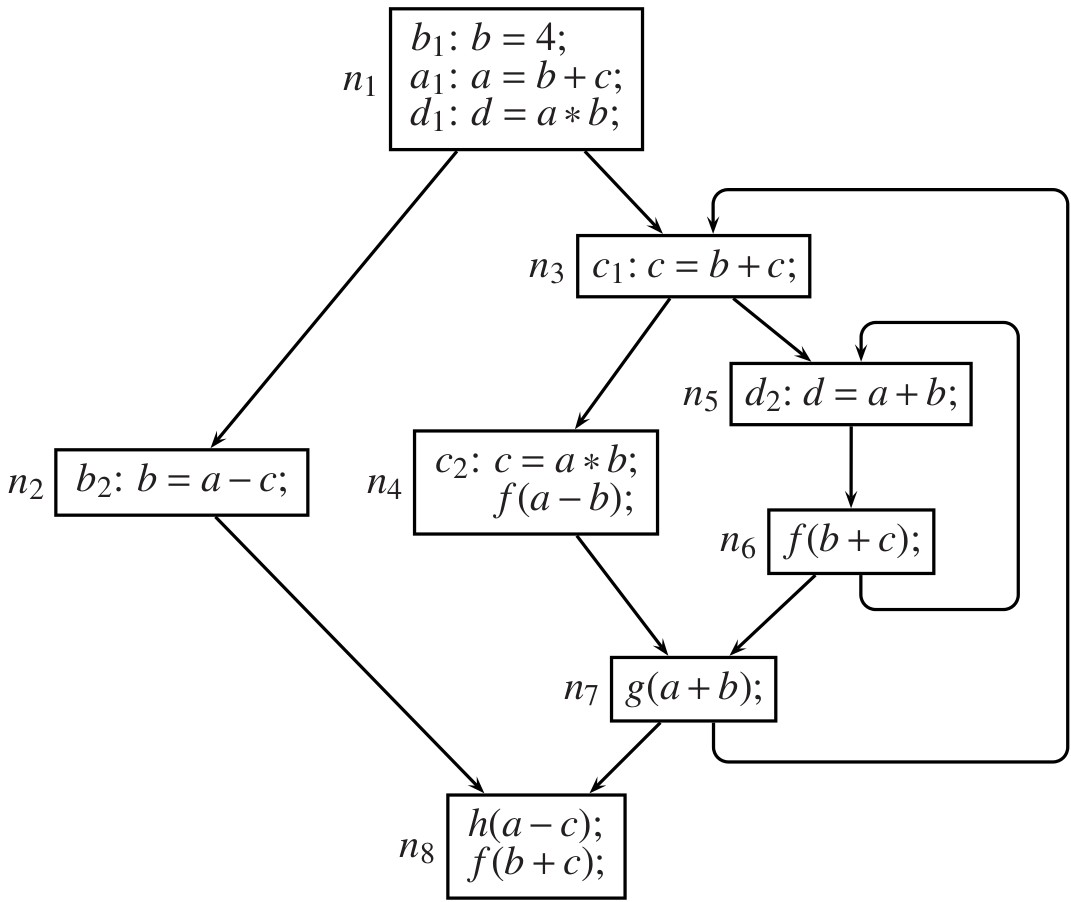
\includegraphics[scale=0.3]{cfg_liveness.png}
	  \caption{Example of CFGraph of a program function \citep{khedker2009data}.}
	  \label{fig:cfg_liveness}
\end{figure}

\begin{table}[]
\begin{tabular}{|c|c|c|c|c|c|c|}
\hline
\multirow{3}{*}{Vertex} & \multicolumn{2}{c|}{\multirow{2}{*}{Local Generation}}  & \multicolumn{4}{c|}{Global Information}                             \\ \cline{4-7} 
                        & \multicolumn{2}{c|}{}                                   & \multicolumn{2}{c|}{Iteration 1} & \multicolumn{2}{c|}{Iteration 2} \\ \cline{2-7} 
                        & $\texttt{gen[}n\ttt{]}$                        & $\ttt{kill[}n\ttt{]}$                   & $\ttt{out[}n\ttt{]}$             & $\ttt{in[} n\ttt{]}$             & $\ttt{out[}n\ttt{]}$             & $\ttt{in[} n\ttt{]}$            \\ \hline
$n_8$                   & $\{a, b, c\}$                & $\emptyset          $            & $\emptyset$               & $\{a, b, c\}$    & $\emptyset          $     & $\{a, b, c\}$    \\ \hline
$n_7$                   & $\{a, b\}$                   & $\emptyset          $            & $\{a, b, c\}$     & $\{a, b, c\}$    & $\{a, b, c\}$     & $\{a, b, c\}$    \\ \hline
$n_6$                   & $\{b, c\}$                   & $\emptyset          $            & $\{a, b, c\}$     & $\{a, b, c\}$    & $\{a, b, c\}$     & $\{a, b, c\}$    \\ \hline
$n_5$                   & $\{a, b\}$                   & $\{d\}      $            & $\{a, b, c\}$     & $\{a, b, c\}$    & $\{a, b, c\}$     & $\{a, b, c\}$    \\ \hline
$n_4$                   & $\{a, b\}$                   & $\{c\}      $            & $\{a, b, c\}$     & $\{a, b\}   $    & $\{a, b, c\}$     & $\{a, b\}   $    \\ \hline
$n_3$                   & $\{b, c\}$                   & $\{c\}      $            & $\{a, b, c\}$     & $\{a, b, c\}$    & $\{a, b, c\}$     & $\{a, b\}   $    \\ \hline
$n_2$                   & $\{a, c\}$                   & $\{b\}      $            & $\{a, b, c\}$     & $\{a, c\}   $    & $\{a, b, c\}$     & $\{a, c\}   $    \\ \hline
$n_1$                   & $\{c\}   $                   & $\{a, b, d\}$            & $\{a, b, c\}$     & $\{c\}      $    & $\{a, b, c\}$     & $\{c\}      $    \\ \hline

\end{tabular}
\caption{Solving the Equation \ref{eq:liveness} for Figure \ref{fig:cfg_liveness} 
\citep{khedker2009data}.}
\label{fig:table_cfg}
\end{table}

\end{subsubsection}

\end{subsection}

\begin{subsection}{Dominator Tree}
	One data structure used on optimization are
	\textit{dominator trees}. First we must define what \textit{domination} means:

	\begin{definition}
		Let $G = (V, E, s_0, F)$ be a Control-Flow Graph and $u, v \in V$. We say
		that $u$ \textbf{dominates} $v$ if every path from $s_0$ to $v$ go through
		$u$.
	\end{definition}

	That means that if some node $u$ dominates $v$, then it is certain that, in
	the current thread, the code in $u$ will be executed before $v$.
	\cite{georgiadis2006finding} presents a forward dataflow equation
	to compute the set of all dominators of a node:


\begin{equation}\label{eq:domtree_dataflow}
\begin{split}
	\texttt{dom[} v \texttt{]} &= 
	\begin{cases}
	  \{v\},& \text{if } v = s_0 \\
	  \left(\bigcap_{p \in \text{pred}(v)}\texttt{dom[}p\texttt{]}\right) \cup \{v\} ,& \text{otherwise} \\
	\end{cases}
\end{split}
\end{equation}

	However, instead of solving Equation \ref{eq:domtree_dataflow}
	every time we want to know if there is such dominance, or avoid
	holding a table containing \textit{every} dominator of a node,
	it is convenient to build a data structure that can quickly query
	such information. Such data structure is the \textit{dominator tree}
	of a CFGraph. Figure \ref{fig:domtree} presents the dominator tree of the CFGraph
	presented in Figure \ref{fig:cfg_liveness}.

\begin{figure}
\centering
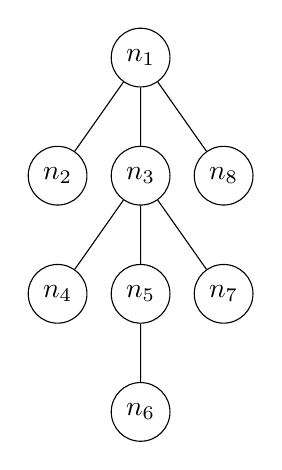
\begin{tikzpicture}[sibling distance=3em,
  every node/.style = {shape=circle,
    draw, align=center}]]
  \node {$n_1$}
    child { node {$n_2$} }
    child { node {$n_3$}
      child { node {$n_4$} }
      child { node {$n_5$}
        child { node {$n_6$} } }
      child { node {$n_7$} } }
  	child { node {$n_8$} };
\end{tikzpicture}
\caption{Dominator tree of Figure \ref{fig:cfg_liveness}}
\label{fig:domtree}
\end{figure}


	Dominator trees are often used to build the Static Single Form (SSA) of a
	CFGraph, to detect loops in the Control-Flow Graph, and in several loop
	optimizations, such as hoisting constant variables outside of a loop,
	detecting induction variables, and so on.
	\cite{appel2004modern} provides algorithms to detect loops using the
	CFGraph, which is useful when the language supports \texttt{goto}s. A
	faster algorithm (but complex than the dataflow equation) algorithms to
	build the Dominator tree of a CFGraph is presented by
	\cite{georgiadis2006finding}.

\end{subsection}

\begin{subsection}{Static Single Assignment Form (SSA)}

Consider the following sequence of statements:
\begin{align}
x &= 2 \nonumber \\
y &= x \times x \nonumber \\
y &= y + 1 \nonumber \\
y &= 1 \nonumber
\end{align}

Clearly, the second and third statements can be discarded, and the first
and last statements can be discarded as well if there is no further use of $x$ and $y$ in the program. However, how can the compiler know that? SSA form makes this clear. The idea is that variables can not be redefined, only new variables can be created, which motivates the following definition.

\begin{definition}
	A program is in SSA form if there is exactly one assignment for each
	variable.
\end{definition}

We can convert the presented sequence of statements in this form by creating
a new variable for each left-hand-side of the assignment. Therefore, if a
variable has multiple definitions, we can eliminate that by creating a new
variable for that value, which yields
\begin{align}
x &= 2 \nonumber \\
y_1 &= x \times x \nonumber \\
y_2 &= y_1 + 1 \nonumber \\
y_3 &= 1 \nonumber
\end{align}

This will lead to the variable $y_2$ being unused because it is nowhere present
on the right-hand side of any assignment (has no use in the \textit{def-use}
chain), meaning that it can be discarded; which will then imply that $y_1$ will
be unused and can be discarded as well.

However, SSA form can get trickier to implement if there are jumps in the
programs, which is often the case with \texttt{if} and \texttt{while}
statements. In Figure \ref{fig:code_normal}, the value of \texttt{u}
depends upon which path the execution was taken, which depends on the
\textit{condition}. The solution fot this is to introduce a $\phi$-function,
which will select the correct variable. Figure \ref{fig:code_ssa_form}
illustrates this.

\begin{figure}[ht]
    \centering
    \begin{subfigure}[b]{0.40\textwidth}

        \begin{lstlisting}[
            language=pseudocode,
            style=pseudocode,
            style=wider,
            functions={},
            specialidentifiers={extern, call},
            ]
            if (condition) then
                a = -1;
            else
                a = 1;
            end
            u = a*v;
        \end{lstlisting}
        \caption{\label{fig:code_normal}}
    \end{subfigure}
    \begin{subfigure}[b]{0.40\textwidth}
        \begin{lstlisting}[
                language=pseudocode,
                style=pseudocode,
                style=wider,
                functions={},
                specialidentifiers={extern, call, PHI},
              ]
            if (condition) then
                $a_1$ = -1;
            else
                $a_2$ = 1;
            end
            $a_3$ = $\phi$($a_1$, $a_2$)
            u = $a_3$*v;
        \end{lstlisting}
        \caption{\label{fig:code_ssa_form}}
\end{subfigure}
\caption{A program (a) and its SSA representation (b)}
\end{figure}

However, this illustration explains little about when to
place $\phi$ functions. A way of determining it is to use
the \textit{dominance frontier criteria}

\begin{definition}
	Let $G = (V, E, s_0, F)$ be a CFGraph and $u, v \in V$. We say that
	$u$ \textbf{strictly dominates} $v$ if $u$ dominates $v$, but
	$u \neq v$. We denote that $u$ idom $v$.
\end{definition}

\begin{definition}
	The \textbf{dominance frontier} of a node $x \in V$ is the set of all nodes $w \in V$
	such that $x$ dominates a predecessor of $w$, but does not strictly dominate $w$ \citep{appel2004modern}.
	Or, in set theory notation:
\end{definition}
\vspace*{-1cm}
	$$\texttt{dfront[}x\texttt{]} = \conj{w \in V}{x \text{ dom } y \text{ for some } y \in \text{pred}(w) \text{ and } y \text{ does not sdom } w}$$

This definition looks blurry, but it can be easily understood as the
\textit{border of nodes where the dominance stops}.  Figure
\ref{fig:dom_frontier} illustrates this concept with a plot of the dominated
nodes of $v_5$ in the beige area and the dominance frontier in the green area.

\begin{figure}[ht]
 \centering
 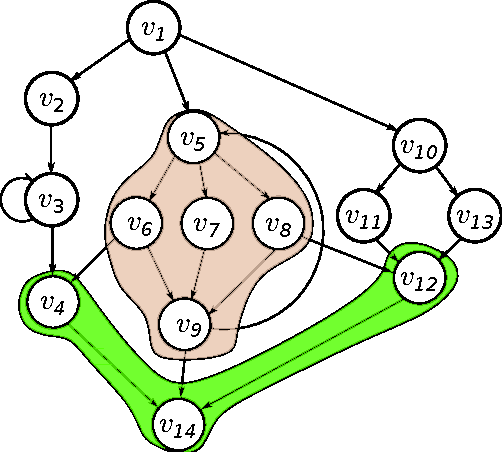
\includegraphics[scale=1.0]{dom_frontier.pdf}
 \caption{Dominance frontier of node $v_5$. Beige is dominated by $v_5$. Green is in dominance frontier of $v_5$.}
 \label{fig:dom_frontier}
\end{figure}

The criteria to place $\phi$-functions are the following: When a node $x$ contains a defintion
of a variable $a$, then any node $z$ in the dominance frontier of $x$ needs a $\phi$ function
for $a$. \citep{appel2004modern}.

SSA makes the optimizing compiler fast because it avoids relying on dataflow
bit vector equations to compute \textit{def-use}. Instead of finding whenether a
certain variable was redefined, or detecting which version of the variable is being
used, SSA simply enforces that a variable has a single definition. This makes
several optimizations easy.

For instance, dead-code elimination can simply check if a variable has no use.
If a variable had previously two definitions and the second has no use, SSA
will transform this variable into two other variables and the second one
would have no use, and therefore could be elminated \citep{appel2004modern}.

\end{subsection}

\begin{subsection}{Callgraphs and Interprocedural Analysis}

Some optimizations require interaction with other functions, one clear example
of this is the \textit{function inlining} optimization. When there is a
function call, the call itself consumes time, and therefore it may be
interesting to copy and paste the content of the function being called and
remove the call at all.  Therefore, a data structure is required to model the
interactions between functions.

That is the purpose of a \textit{Callgraph}: each vertex denotes a function,
and each edge represents a call between two functions. 

\begin{definition}
	A Callgraph is a graph $G = (V, E)$, where $V = \{f_1, f_2, \cdots, f_{|V|}\}$
	are the set of functions, and $E = \conj{(u, v)}{u, v \in V}$ are the set
	of edges representing a function call. Given $(u, v) \in E$, this means
	that $u$ (the \textbf{caller}) calls $v$ (the \textbf{callee}).
\end{definition}

Figure \ref{fig:call_graph} gives an example of a Callgraph. When applying
Interprocedural Optimizations, each vertex can also hold some sort of
\textit{summary} of the function instead of the entire function, because the
program being compiled often is large enough that there is not sufficient
memory to hold the contents of the functions in the host machine which is
compiling the code. This is the case when working with
the Link Time Optimization (LTO) technique.

There are some extensions to the dataflow frameworks to work on Interprocedural
Optimizations \citep{khedker2009data}, however, they require complete
information about the function in memory, which may not be present in this
stage on compilers such as GCC \citep{gcc_ipa}.

\begin{figure}[ht]
\centering
  \begin{subfigure}[b]{0.40\textwidth}
      \begin{lstlisting}[
        language=pseudocode,
        style=pseudocode,
        style=wider,
        functions={},
        specialidentifiers={extern, call},
      ]
        extern function g,h

        function f()
            call $g$
            call $h$
        end

        function main()
            call $f$
            call $h$
        end
      \end{lstlisting}
  \end{subfigure}
  \begin{subfigure}[b]{0.40\textwidth}
    \tikzstyle{line} = [draw, -latex]
    \tikzstyle{node} = [draw, circle]
    \begin{center}
    \scalebox{1.0}{
    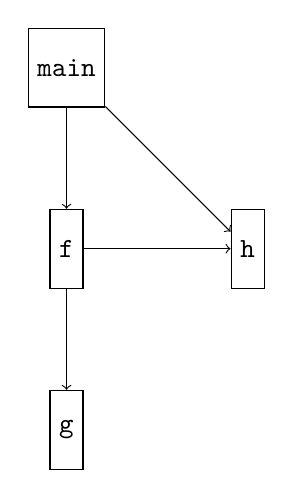
\begin{tikzpicture}[node distance = 2.3cm, minimum height = 1cm, auto]
        % Place nodes
        \node [node]                    (main) {\texttt{main}};
        \node [node, below of = main]        (f) {\texttt{f}};
        \node [node, below of = f]           (g) {\texttt{g}};
        \node [node, right of = f]           (h) {\texttt{h}};

        % Draw edges
        \draw[->]    (main)           -- (f);
        \draw[->]    (f)              -- (g);
        \draw[->]    (f)              -- (h);
        \draw[->]    (main)           -- (h);
    \end{tikzpicture}
    }
    \end{center}
  \end{subfigure}
  \caption{A program and its callgraph}
  \label{fig:call_graph}
\end{figure}

Callgraphs are often used to model interprocedural optimizations, such as
function inlining, as it models the call relationship between functions. For
instance, inlining can increase the program size in bytes tremendously if the
function is called from multiple locations, which can further slow down the
program due to instruction cache and page faults.

\end{subsection}

\begin{subsection}{Register Allocation}
Registers are very fast, but small memories inside a processor, which data is
required to be loaded for operations like add, subtract, multiply, etc. These
memories are a very scarce resource in a processor, and therefore it
must be administered carefully.

A good (near-optimal) register allocation can hugely speed up the program
because it avoids unnecessary accesses between the CPU and the computer's
memory, and this is the purpose of the register allocation.

The idea of this step is to represent the variables in the IR so that it can be
easily mapped into the CPU registers. Therefore, since the IR can have an
infinite number of variables, the goal here is to rewrite the code such that it
uses no more temporaries than there are registers in the machine. For example,
consider the Figure \ref{fig:register_ir}. In (a), we have a sketch of the
program, and in (b) we have the rewrite using at most 4 registers.

\begin{figure}[ht]
    \centering
    \begin{subfigure}[b]{0.40\textwidth}
		\begin{align}
			a &= b + c      \nonumber \\
			d &= a \times e \nonumber \\
			f &= d + 1      \nonumber
		\end{align}
        \caption{\label{fig:code_normal}}
    \end{subfigure}
    \begin{subfigure}[b]{0.40\textwidth}
		\begin{align}
			r_1 &= r_2 + r_3      \nonumber \\
			r_1 &= r_1 \times r_4 \nonumber \\
			r_1 &= r_2 + 1        \nonumber
		\end{align}
        \caption{\label{fig:code_register}}
\end{subfigure}
\caption{A program (a) and its presentation on registers (b)}
\label{fig:register_ir}
\end{figure}

	However, how can a compiler \textit{know} when a certain variable will not
	be used anymore, and we can replace the register with computation of some
	kind? By using the \textit{liveness analysis}.

\begin{definition}
	Let $t_1$ and $t_2$ be two temporaries variables. If $t_1$ and
	$t_2$ are live at a given point $p$, then $t_1$ and $t_2$ can not
	share the same register.
\end{definition}

This information is used to build an \textit{interference graph}, which an
example is presented in Figure \ref{fig:interf_graph}.

\begin{definition}
	An interference graph $G = (V, E)$ is a graph where $V = \mathbb{V}$ is the
	set of variables in the program, and $E \ssq V \times V$ are the set of
	edges. An edge $(u, v) \in E$ if $u$ and $v$ are simultaneously live at
	at some program point $p$.
\end{definition}

\begin{figure}
    \tikzstyle{line} = [draw, -latex]
    \tikzstyle{node} = [draw, circle]
    \begin{center}
    \scalebox{1.0}{
    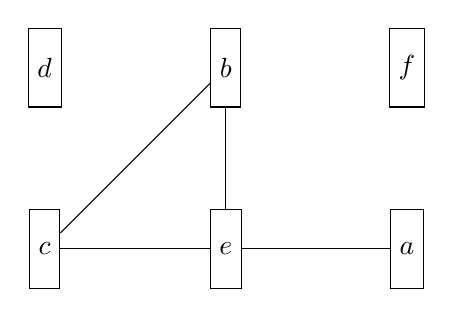
\begin{tikzpicture}[node distance = 2.3cm, minimum height = 1cm, auto]
        % Place nodes
        \node [node]                         (d) {$d$};
        \node [node, right of = d]           (b) {$b$};
        \node [node, right of = b]           (f) {$f$};
        \node [node, below of = d]           (c) {$c$};
        \node [node, right of = c]           (e) {$e$};
        \node [node, right of = e]           (a) {$a$};

        % Draw edges
        \draw        (b)              -- (c);
        \draw        (c)              -- (e);
        \draw        (e)              -- (b);
        \draw        (e)              -- (a);
    \end{tikzpicture}
    }
    \end{center}
	  \caption{Interference Graph of Figure \ref{fig:register_ir}.}
	  \label{fig:interf_graph}
\end{figure}

After the interference graph is constructed, it is possible to know how many
registers it is necessary and where to allocate once the graph is colored.
Graph coloring, unfortunately, is an NP-Complete problem
\citep{karp1972reducibility}, which implies that a heuristic is necessary to
solve this problem.

\cite{appel2004modern} shows one heuristic. Suppose that the target machine has
$k$ available registers. Once the interference graph has been built, select one
node $v$ with degree $d(v)$ such that $d(v) < k$. The idea is around the fact that
if $G' = G - \{v\}$ can be colored, then so do $G$ because one can simply select
a color distinct from every node that $v$ is adjacent to, which results in a 
recursive coloring algorithm. This is called \textit{simplify}.

However, nothing is preventing that there are no nodes $v$ such that
$d(v) \geq k$. In this case, there is no alternative other than allocate the
variable in memory. This is called \textit{spilling}.

Once this process is completed, variables can be renamed accordingly to their
register, or memory location.

\end{subsection}

\begin{subsection}{Instruction Selection}
An important step in the final translation process is the
\textit{instruction selection}. Most processors (such as x86) have more
than a way to translate a statement to machine code, for instance, 
assigning a variable to zero. One could use \texttt{mov reg, 0}, or
even \texttt{xor reg, reg}, but the latter one is faster as it takes fewer
cycles to execute. This is specially important for CISC-based processors,
which a sequence of instructions can be replaced with a single instruction,
resulting in a faster program. Detecting such cases is the main issue here.

There are several techniques to select instructions. One of the simplest
is the \textit{macro translation}, where each statement is replaced
by the final code locally for each line of the IR. This has the advantage
of being a fast way to implement a way to translate the code, but
very often generate poor final code, as illustrated in
Figure \ref{fig:macro_exp}. Some optimizations can be employed
to improve the result of such translations, such as
\textit{peephole optimization}, which search in a small window unnecessary memory operations that annulate themselves.

\begin{figure}
\tikzstyle{block} = [rectangle, draw, fill=white,
    text width=15em, text centered, rounded corners, node distance = 1cm and 1cm, auto, minimum height=2em]
\tikzstyle{line} = [draw, -latex]
\tikzstyle{cloud} = [draw, ellipse,fill=white, node distance=2cm,
    minimum height=2em]

\begin{center}
\scalebox{0.8}{
\begin{tikzpicture}
    % Place nodes
    \begin{scope}[node distance = 1cm and 5cm]
    \node [block]                  (c1) {$\textit{fib}_i = \textit{fib}_{i-1} + \textit{fib}_{i-2}$};
    \node [block, below=of c1]     (c2) {$\textit{fib}_{i-2} = \textit{fib}_{i-1}$};
    \node [block, below=of c2]     (c3) {$\textit{fib}_{i-1} = \textit{fib}_{i}$};
    \end{scope}

    \node [block, right=of c1]     (asm1) {\texttt{mov eax, DWORD [ebp-8]} \\ \texttt{mov ebx, DWORD [ebp-12]} \\ \texttt{add eax, ebx} \\ \texttt{mov [ebp-4], eax}  };
    \node [block, right=of c2]     (asm2) {\texttt{mov eax, DWORD [ebp-8]} \\ \texttt{mov [ebp-12], eax}};
    \node [block, right=of c3]     (asm3) {\texttt{mov eax, DWORD [ebp-4]} \\ \texttt{mov [ebp-8], eax}};

    % Draw edges
    \draw[->]    (c1.east)        -- (asm1.west);
    \draw[->]    (c2.east)        -- (asm2.west);
    \draw[->]    (c3.east)        -- (asm3.west);
\end{tikzpicture}
}
\end{center}
\caption{Macro instruction selection for x86. Intel syntax.}
\label{fig:macro_exp}
\end{figure}

Another approach is to treat the IR as a \textit{tree}, then try to
pattern-match a set of nodes in which this pattern has an efficient
translation.  Figure \ref{fig:tree-matching} illustrates this process, in
general.

\begin{figure}
\centering
	 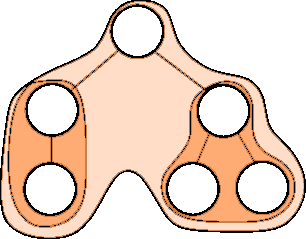
\includegraphics[scale=1.0]{tree_replace.pdf}
	  \caption{Illustration of a tree-matching algorithm}
	  \label{fig:tree-matching}
\end{figure}

There are some algorithms for matching such trees. One, proposed by
\cite{glanville1978}, describes a Context-Free Grammar to translate the IR into
assembler language. However, in many machines, such grammar will always be
ambiguous, implying that such grammars will not pass the $\mathcal{DK}_1$ test
(see Section \ref{sec:bottom-up}), either by \textit{shift-reduce} or
\textit{reduce-reduce} conflicts.

	The solution of this problem is as follows:

	\begin{itemize}
		\item On \textit{shift-reduce} conflicts, always choose to shift. The intuition is that larger patterns will result in more optimal code since it allows more information to be gathered by the parser. However, the parser could simply select to \textit{shift} when it should have 	\textit{reduce}d. Therefore, either backtracking is necessary here when the parser takes the wrong decision, or the grammar designer provides additional rules to avoid such cases.

\item On \textit{reduce-reduce} conflicts, it selects the rule with yields the
longest pattern. The reason is also that the longest patterns will generate
better code. However, even this can also result in a parsing error. The
solution is to devise a rule in which can be used as a fallback, and the
authors provide a way to automatically find such a rule.

	\end{itemize}

Such parsers are very interesting because, given a way to express what the
parser should produce and the cost of these productions, one can quickly
implement a new \textit{backend} to the compiler.  The main issue, however, is
the high number of states required by the
parser \citep{blindell2016instruction}, which often turns it impractical.

There is a way to optimally select instructions on a tree using a technique
called \textit{dynamic programming} \citep{ripken1977formale}. The idea is that given a node $n$, it is enough to first consider to minimize the cost
of the child and then try to minimize the cost of $n$. Mathematically, let
$P_n$ the set of patterns possible to be applied to $n$. Therefore, the
minimal cost $\texttt{PD[}n\texttt{]}$ is:

\[
    \texttt{pd[}n\texttt{]} =
     \begin{cases}
       \min_{p \in P_n} \texttt{cost[}p\texttt{]}  &\quad\text{if } n \text{ is leaf}\\
       \min_{p \in P_n} \texttt{cost[}p\texttt{]} + \sum_{f \in \text{succ}(p)} \texttt{pd[}f\texttt{]} &\quad\text{otherwise}\\
     \end{cases}
\]

Another way of selecting instructions is through Directed Acyclic Graph. Its
advantage, when compared to trees, is that it can represent common
subexpressions, but unfortunately optimal algorithms for this representation
are NP-complete \citep{koes2008near}. The majority of techniques employed here
are greedy, as in \cite{llvm_insn_selection}.

Finally, a more detailed discussion on instruction selection is presented
by \cite{blindell2016instruction}.

\end{subsection}

\end{section}

\begin{section}{Software Engineering in Compilers}\label{sec:engineering}

%Para evitar confusões a respeito das diferentes linguagens que um compilador
%trabalha em seus muitos estágios, é adotado a seguinte nomenclatura neste trabalho:
%Denote \textit{Linguagem Fonte} como sendo a linguagem
%na qual o código fonte do programa a ser compilado foi originalmente escrito;
%\textit{Linguagem Intermediária} uma das linguagens internas do compilador; e
%\textit{Linguagem Alvo} a linguagem na qual o compilador deverá gerar código.


%Compiladores são grandes projetos destinados a tradução de códigos fonte
%entre distintas linguagens de programação. Normalmente, compiladores traduzem
%linguagens de alto nível, como C, para linguagens mais próximas da máquina,
%como a linguagem de montagem - embora isso não seja uma regra pois existem
%compiladores cuja única tarefa é realizar uma tradução entre duas linguagens
%de alto nível.

%Compiladores também costumam otimizar
%o código que passam por eles, aplicando diversas heurísticas de
%maneira a acelerar o código a ser produzido, substituindo trechos de código por
%outros mais eficientes, reordenando as instruções do programa, etc.

Compilers are large programs. Because of this, there is a great interest in
avoiding rewriting a compiler when a new language is proposed, or when new
hardware is created. For that, compiler writers usually adopt the following
modularization \citep{redhat} \citep{llvm}, as illustrated by Figure
\ref{fig:compiler_arch}:

%Por serem programas extremamente grandes, existe um grande interesse em evitar
%reescrever um novo compilador
%sempre que uma nova linguagem é proposta, ou um novo \textit{hardware} é criado.
%Para isso, a seguinte modularização é largamente adotada por projetistas de
%compiladores \citep{redhat} \citep{llvm}, conforme ilustrado na Figura \ref{fig:compiler_arch}:
%

\begin{itemize}

\item A Front End for each Source Language. In this module are executed the
lexical and syntactical analysis to construct the Abstract Syntax Tree (AST)
and populating the Symbol Table. Following that, this structure is converted to
another compiler's IR.

\item A Middle End, responsible for applying several \textit{hardware independent}
optimizations to the already converted IR code. A \textit{hardware independent}
optimization is such that there are no dependency with regard to the Target
Language (often, assembler of some processor). Example: \textit{constant propagation}.

\item A Back End for each Target Language, responsible to translate the IR to
the Target Language and applying \textit{hardware dependent} optimizations,
such as register allocation and instruction selection. A \textit{hardware dependent}
optimization is such that there \textit{is} a dependency with regard to the
Target Language. Example: \textit{register allocation}.

\end{itemize}

%\begin{itemize}
%    \item Um \textit{Front End} para cada Linguagem Fonte.
%	Neste módulo são executadas as análises léxica e sintática, com a
%        finalidade de construir uma Árvore de Sintaxe Abstrata (AST), para que em
%seguida, ela seja convertida para uma Linguagem Intermediária do compilador.
%
%    \item Um \textit{Middle End}, responsável por aplicar diversas otimizações
%independentes de arquitetura no código já convertido para a Linguagem Intermediária.
%
%    \item Um \textit{Back End} para cada linguagem alvo, responsável por converter a linguagem intermediária
%na linguagem alvo. Aqui outras otimizações específicas da linguagem alvo são realizadas,
%como alocação de registradores e seleção de instruções.
%\end{itemize}

However, this modularization is completely optional: older compilers destined
to simply doing a direct translation between languages, such as the UNIX C
Compiler, do not have an IR \citep{ritchie1979tour}. Not only that, several
textbooks about compilers do not mention the Middle-End part, being a part of
the Back-End of the compiler \citep{dragonbook}. Not adopting this
modularization simplifies the project, but also complicates the insertion of
new programming languages, as well as adding support to new hardware.

%Porém, essa modularização é opcional: compiladores mais antigos destinados a fazer uma
%conversão direta entre duas linguagens, como o UNIX C Compiler, não costumam usar uma linguagem
%intermediária \citep{ritchie1979tour}, além de diversos livros-texto não mencionarem tal módulo, fundindo suas
%funcionalidades com o \textit{Back End} \citep{dragonbook}. Não adotar tal metodologia
%simplifica o projeto, mas dificulta a inserção de suporte a novas
%linguagens de programação.


\begin{figure}
\tikzstyle{block} = [rectangle, draw, fill=white,
    text width=6em, text centered, rounded corners, node distance=5cm, auto, minimum height=2em]
\tikzstyle{line} = [draw, -latex]
\tikzstyle{cloud} = [draw, ellipse,fill=white, node distance=2cm,
    minimum height=2em]

\begin{center}
\scalebox{0.8}{
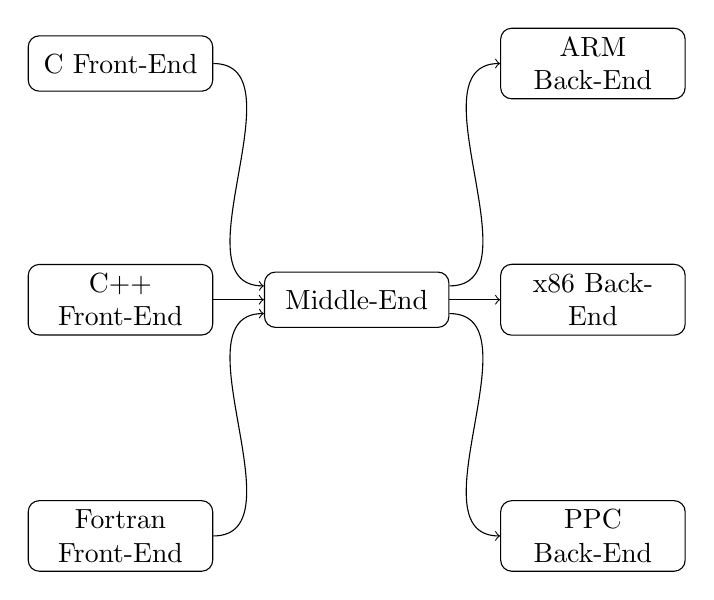
\begin{tikzpicture}[node distance = 3cm, auto]
    % Place nodes
    \node [block]                      (front_c)    {C Front-End};
    \node [block, below of=front_c]    (front_cpp)  {C++ Front-End};
    \node [block, below of=front_cpp]  (front_fort) {Fortran Front-End};
    \node [block, right of=front_cpp]  (middle)     {Middle-End};
    \node [block, right of=middle]     (back_x86)   {x86 Back-End};
    \node [block, above of=back_x86]   (back_arm)   {ARM Back-End};
    \node [block, below of=back_x86]   (back_ppc)   {PPC Back-End};


    \coordinate [left of=front_c]    (c_code);
    \coordinate [left of=front_cpp]  (cpp_code);
    \coordinate [left of=front_fort]  (fort_code);

    \coordinate [right of=back_x86] (x86_code);
    \coordinate [right of=back_arm] (arm_code);
    \coordinate [right of=back_ppc] (ppc_code);

    % Draw edges
    \draw[->]    (front_c.east)     to [out=0,in=180] ([yshift=0.5em]  middle.west);
    \draw[->]    (front_cpp.east)   to [out=0,in=180] (middle.west);
    \draw[->]    (front_fort.east)  to [out=0,in=180] ([yshift=-0.5em] middle.west);

    \draw[->]    ([yshift=-0.5em] middle.east)  to [out=0,in=180] (back_ppc.west);
    \draw[->]    (middle.east)                  to [out=0,in=180] (back_x86.west);
    \draw[->]    ([yshift=0.5em] middle.east)   to [out=0,in=180] (back_arm.west);

    %\draw[->]    (sintatico.west)   -- (lexico.east)    node[midway] {próximo\_token()};
    %\draw[->]    (fonte.west)       -- (lexico.west)    node[pos=0, above] {Código Fonte};
    %\draw[->]    (sintatico.east)   -- (ast.west)       node[pos=1, above] {Árvore Abstrata};
\end{tikzpicture}
}
\end{center}

\caption{Compiler Architecture}
\label{fig:compiler_arch}
\end{figure}

%\begin{subsection}{\textit{Front-End}}
\begin{subsection}{Front-End}

A Front-End is a module responsible for direct interaction with the code
written in the Source Language, which means from a Software Engineering
perspective, for adding support to a new Source Language, it is enough to write
a new Front-End. It is also possible that some classes are shared between
frontends, which may be the case of a compiler that supports both C and C++.

%Um \textit{Front End} é um módulo responsável por interagir diretamente com o
%código escrito na Linguagem Fonte a ser compilado. Ele costuma ser único
%para cada Linguagem Fonte, ou seja, para inserir suporte a uma nova
%Linguagem Fonte, basta implementar um novo \textit{Front End}, mas é
%possível que algumas classes sejam
%compartilhadas, como no caso de um compilador que dê tanto para C quanto para e C++.


As a first step, the Front-End performs a lexical and syntactical analysis for
generating an AST and verify if the input text belongs to the language. It is
also responsible for printing parsing errors in a way that the user can easily
understand them. The Front-End also populates the Symbol Table of the compiler
with symbols that it has seen so far when compiling the program for checking if
there are references to undefined symbols. These three pieces (the Lexical
Analyser, the Syntactic Analyser, and the Symbol Table) frequently communicate
with each other, as illustrated in Figure \ref{fig:lexico_sintatico}.

%Como primeiro passo, \textit {Front End} realiza uma análise
%léxica e sintática, com a finalidade de gerar uma AST e verificar
%se o texto dado como entrada realmente pertence à linguagem.
%Estes dois analisadores se comunicam constantemente, conforme ilustrado na Figura
%\ref{fig:lexico_sintatico}.


%    Primeiro, a análise léxica é responsável por ler o arquivo
%de texto contendo o código fonte, e quebrar as palavras em \textit{tokens}, que
%serão alimentados para o analisador sintático. Por consequência, ele é capaz de
%realizar alguns filtros, \textit{e.g}. ignorar os comentários, identificar constantes
%numéricas, eliminar espaços desnecessários, e substituir um \textit{token} por
%outro.
%Analisadores léxicos também podem ser usados para substituição
%de macros, como implementado pelo preprocessador do C
%(CPP)\footnote{https://gcc.gnu.org/onlinedocs/cppinternals/Lexer.html}.

%Geralmente, os Analisadores Léxicos são implementados utilizando autômatos
%por diversos motivos, entre eles sua atrativa complexidade computacional
%$O(n)$, onde $n$ é o tamanho da entrada, pela existência de algoritmos
%para converter expressões regulares em autômatos \citep{thompson}, e pela
%existência de algoritmos para minimização de estados de um autômato
%\citep{hopcroft1971n}. Isto possibilita que geradores de analisadores léxicos
%como o \texttt{Flex}\footnote{https://www.gnu.org/software/flex/}
%sejam bastante eficientes.

After the AST is generated and the Semantic Analysis is completed, it is often
converted to an IR, where Target-Independent Optimizations are performed. This
yields the control to the Middle-End of the compiler.

\end{subsection}

\begin{subsection}{Middle End}

The Middle-End is responsible to work on one or more IR(s) of the compiler. If
there are checks which can be postponed in the Front-End to this stage, it is
preferable, once it avoids these checks on every Source Language's Front-End.

Here, we construct data structures in which might be necessary for the
hardware-independent optimizations, such as the Control-Flow Graph, the
Callgraph, the SSA representation, and so on. After that, the compiler indeed
runs these optimizations.

The Middle End is where the most effort is spent in development. Every new
optimization here will improve the code for every target machine that the
compiler supports.

After this optimization process, the code in this IR can be further transformed
into other IR to something that is more closely related to the target hardware.
After that, the control is passed to one of the compiler's Back End, where it
will be transformed to the final language.

\end{subsection}

\begin{subsection}{\textit{Back End}}

The \textit{Back End} is responsible for the final translation to the target
language, as well as hardware-dependent optimizations. Therefore, it is also
responsible for selecting instructions optimally (or close to) as well as
selecting registers from the best way possible for the program's variable.

The Back End should be implemented in a way that it can simply be switched for
another without any modification to the Middle End. With this, the code can be
easily compiled to another target language.

After the Back End has done its processing, the final code is issued and the compilation is complete.

\end{subsection}

\begin{subsection}{Compilation Passes}

Compilers, however, can optimize for several metrics, not only execution time.
Industrial compilers also very often support \textit{optimization for size} for
embedded systems, or even \textit{optimize for power consumption}, which can be
interesting for both embedded systems and data centers. Therefore, some
optimizations may be executed while others must be disabled depending on what
are you optimizing to. This is where a simple but powerful modularization comes
into, the \textit{compiler passes}.

A pass is simply a set of rules to run in the IR. For instance, one pass
could match and replace a set of statements in the IR for a faster one,
or even simply collect information about some function, such as the
\textit{cyclomatic complexity}.

Passes can be easily implemented using classes, and all passes are structured
in a queue. Each pass should receive the information in which it is working on
(for instance, a data structure representing the current function being worked
on) and has a \textit{gate} method, which will determine if this optimization
will or will not be run, according to some compilation flags or even with some
information collected with some previous pass. It is even possible that there
are subpasses to a pass, containing its own queue of passes. Figure \ref{fig:pass_queue}
illustrates this queue. 

\begin{figure}

\tikzstyle{block} = [rectangle, draw, fill=white,
    text width=6em, text centered, rounded corners, node distance=5cm, auto, minimum height=2em]
\tikzstyle{line} = [draw, -latex]
\tikzstyle{cloud} = [draw, ellipse,fill=white, node distance=2cm,
    minimum height=2em]

\begin{center}
\scalebox{0.8}{
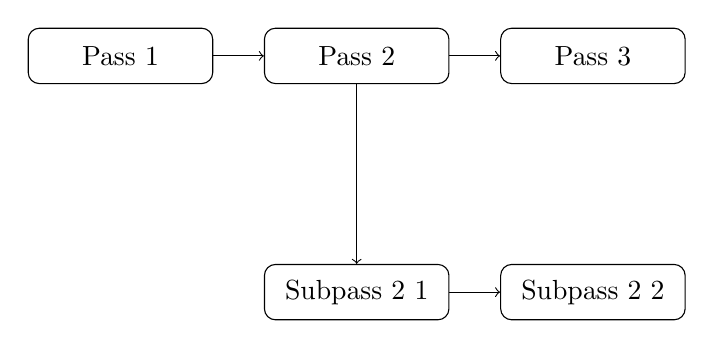
\begin{tikzpicture}[node distance = 3cm, auto]
    % Place nodes
    \node [block]                      (pass1)    {Pass 1};
    \node [block, right of = pass1]    (pass2)    {Pass 2};
    \node [block, below of = pass2]    (subpass1)    {Subpass 2 1};
    \node [block, right of = subpass1] (subpass2)    {Subpass 2 2};
    \node [block, right of = pass2]    (pass3)    {Pass 3};

    % Draw edges
    \draw[->]    (pass1.east)     to [out=0,in=180] (pass2.west);
    \draw[->]    (pass2.east)     to [out=0,in=180] (pass3.west);
    \draw[->]    (pass2.south)    to  (subpass1.north);
    \draw[->]    (subpass1.east)  to [out=0,in=180] (subpass2.west);
\end{tikzpicture}
}
\end{center}
\caption{Pass Queue}
\label{fig:pass_queue}
\end{figure}

\end{subsection}
\end{section}

\begin{section}{The GCC Compiler}\label{sec:gcc_compiler}

The GNU Compiler Collection, also known as GCC, is a project started by
Richard Stallman with the first public release in March of 1987. Back then,
it only supported C language but already allowed code generation for
several architectures \citep{gcc_first_ver}.

Today, GCC supports several source languages, such as C, C++, Fortran, Go, Ada;
and several architectures, such as i386, amd64, riscv, arm, ppc, and pdp-11.
GCC is also an optimizer compiler, which means it can modify the input code to
generate a more efficient version without changing the program semantic. This
is archived through its several IR: GENERIC, GIMPLE, and RTL. The compiler run
optimization passes on each of these IR.

%Hoje, o GCC fornece suporte a diversas Linguagens Fonte como C, C++, Fortran, Go, Ada,
%e várias arquiteturas, como i386, amd64, riscv, arm, ppc, pdp-11. O GCC também
%é um compilador otimizador, ou seja, ele é capaz de alterar o código fornecido
%pelo usuário com a finalidade de gerar código mais eficiente, sem alterar a semântica do programa. Isso é
%possível por conta das várias Linguagens Intermediárias implementadas no
%GCC: GENERIC, GIMPLE, e RTL. O compilador executa vários
%passos de otimização em cada uma dessas linguagens intermediárias.

\begin{subsection}{GENERIC}

GENERIC is a IR that allows to represent any function in the program with
trees.  Such language is a superset of all functionalities and attributes
that every Source Language has, for instance, attributes such as
\texttt{volatile} in C, C++, or even Fortran matrix sum or product. Other
functionalities are more common to every language, such as function calls,
variable declaration, class, expressions, statements, and others
\citep{generic}.

%    O GENERIC é uma linguagem intermediária que possibilita representar quaisquer
%funções do programa através de árvores. Tal linguagem é um superconjunto
%das funcionalidades e atributos que cada Linguagem Fonte contém, por exemplo, atributos
%como \texttt{volatile} de C e C++ contém uma representação nessa linguagem.
%Outras funcionalidades são: chamadas de função, declaração de variáveis, classes,
%funções, expressões, entre outros \citep{generic}.

This language contains a faithful representation of the program closest to what
was written by the programmer, meaning that there are no modifications in the
program. This language is not in 3AC or SSA form, it is only there for an easy
translation to GIMPLE, the hardware-independent IR of GCC in which most
optimizations are done, and to make the development of a Front End easily.
However, that does not mean that optimizations can not be applied here.

There is a match-and-replace mechanism in GCC supporting GENERIC. This
mechanism is very simple: it searches for a chain of statements in the IR for a
pattern and then replaces for another. Such patterns are expressed in the file
\texttt{gcc/match.pd}. This simple mechanism allows several bitwise logic and
mathematical simplifications that can give a significant speedup in the code in
particular cases \citep{sinatan}.


%    Essa linguagem contém uma representação mais próxima de como o programa foi
%escrito pelo programador, ou seja, não são feitas modificações nas expressões.
%Sendo assim, essa linguagem
%intermediária não se enquadra nas categorias de \textit{Three Address Code},
%ou \textit{Static Single Assignment} pois isso demanda modificações no código.
%O objetivo principal dessa linguagem
%é facilitar a tradução para a próxima linguagem intermediária, a GIMPLE, e assim
%facilitar o desenvolvimento dos \textit{Front End} do compilador, mas isso não
%significa que otimizações não possam ser aplicadas aqui.

%    O GCC possui um mecanismo de substituição de nós em sua representação
%interna, dando suporte a árvore construída em GENERIC. Esse mecanismo é simples: o
%compilador procura por uma cadeia de nós na árvore, buscando padrões,
%como especificado no arquivo \texttt{gcc/match.pd}, e os substitui pelo o que
%foi instruído na regra de substituição. Esse mecanismo, embora simples, permite
%com que diversas simplificações matemáticas sejam implementadas no código, o
%que pode significar uma melhora de até $10\times$ em casos particulares
%\citep{sinatan}.

	Finally, each Front End of GCC is responsible for translating the source
	code for this intermediate language. To visualize a program in this representation,
	compile the program with the flag \texttt{-fdump-tree-original}. However,
	the documentation is very clear that C and C++ frontends translate
	directly to GIMPLE \citep{gimple}.

\end{subsection}

\begin{subsection}{GIMPLE}

GIMPLE is another IR from GCC, basically consisting of conversion from GENERIC
to a 3AC representation, having a further step into lowering this
representation to construct the Control-Flow Graph and the SSA form. As
GENERIC, GIMPLE is general enough to represent every attribute from all Source
Languages supported by the compiler. This representation is based on SIMPLE, an
IR from McCAT compiler \citep{gimple}.

%O GIMPLE é outra linguagem intermediária do GCC, basicamente consistindo na
%conversão de GENERIC para \textit{Three Address Code}, havendo ainda um passo
%posterior adicionando uma representação SSA a esta linguagem. Assim como o
%GENERIC, a GIMPLE também é geral o suficiente para representar os atributos
%de todas as Linguagens Fonte de cada \textit{Front End}.  Essa linguagem
%intermediaria é baseada na linguagem SIMPLE, do compilador McCAT \citep{gimple}.

It is in GIMPLE that all hardware-independent optimizations are performed.
GIMPLE has an \textit{Application Programming Interface} (API) for interacting
with statements, tree nodes, the Control-Flow Graph, SSA nodes, and the
Callgraph. GIMPLE has two states, the ``high'' state, with lexical scopes and
nested expressions, and ``low'' state, exposing all implicit jumps and
Exception Handles (EH) regions, removing the lexical scopes, merging similar
return statements, and convert try-catch control flows to exception regions.

GIMPLE code can be dumped by using the flag \texttt{-fdump-tree-gimple},
or even \texttt{-fdump-tree-ssa} to write the SSA representation on the
disk.

\end{subsection}

\begin{subsection}{Register Transfer Language}

	The last IR of GCC is the \textit{Register Transfer Language} (RTL).
	The syntax of this language ressembles Lisp, where expressions
	are represented by a list of commands \citep{rtl}.


%    Por fim, a última linguagem intermediária do compilador GCC é a
%\textit{Register Transfer Language} (RTL). A sintaxe dessa linguagem
%tem inspiração no Lisp, onde as expressões são representadas por uma
%lista de comandos .

	RTL is a language that aims to be as close as the assembler language
	as possible, while still being generic enough to be compatible with
	every target language of GCC. It represents a machine with an infinite
	number of registers that will be correctly selected to a machine
	register on the register allocation pass, or allocated in memory.

%    A RTL é uma linguagem que visa ser extremamente próxima da linguagem
%de montagem, mas ainda sendo genérica o suficiente a ponto de ser compatível
%com todas as Linguagens Alvo do GCC.
%Para isso, ela representa uma máquina com infinitos
%registradores, que serão alocados em registradores reais no passo correspondente.
%Caso a arquitetura alvo não tenha o número necessário de
%registradores, as variáveis deverão ser guardadas em memória. Por exemplo,
%no caso do i386, elas deverão ser salvas na pilha. Esse processo é conhecido
%como \textit{Register Spilling}.

	The final step is the assembler emission once all optimizations were
	performed in RTL. This will employ a macro translation instruction
	selection algorithm to convert RTL functions, statements, and expressions
	into assembler. That is why RTL optimizers are necessary here, to avoid
	generating very poor assembler code \citep{gcc_insns_selection}.

%    Essa é a última Linguagem Indermediária antes da geração do código final. O
%\textit{Back end} transformará o código nessa linguagem para a Linguagem Alvo
%substituindo uma sequência de instruções em RTL por uma sequência de instruções
%na Linguagem Alvo. Essa escolha segue um sistema
%de custos no qual o compilador procura escolher uma sequência de instruções
%que minimiza a soma do custo total da tradução.
%
%    Na arquitetura i386, as regras de substituição estão implementadas
%em \texttt{gcc/config/i386/i386.md}, com o sistema de custos definido
%na \texttt{struct processor\_costs}, no arquivo \texttt{gcc/config/i386/i386.h}.
%Cada processador da arquitetura i386 deve definir o custo de cada instrução,
%como definido em \texttt{gcc/config/i386/x86-tune-costs.h}.


\end{subsection}

\begin{subsection}{Optimization Passes}\label{sec:opt_passes}
	GCC has several optimization passes that are applied to each intermediary
	language. The optimization passes queue is described in
	\texttt{gcc/passes.def}. There are three types of passes:

    \begin{enumerate}
        \item \textbf{IPA} - An Interprocedural pass. This pass operates on the
		callgraph of the program being compiled. These often three step passes:
		on the first run it collect a \textit{summary} of the function, then
		it will \textit{analyze} the callgraph with this summary (for instance,
		to determine if inlining a certain function will not blow the code's size),
		then finally it will \textit{transform} the code. The reason behind this
		that the \textit{analyse} phase must be able to run without having the
		entire function loaded in memory.

        \item \textbf{GIMPLE} - A Hardware-Independent Intraprocedural pass.
		This can do some analysis in the code (such as collecting some metric)
		or even do a deep transformation in the program. One example is
		the \texttt{pass\_vectorize}, which tries to find vectorizable operations
		in the code. It operates on GIMPLE.

        \item \textbf{RTL} - A Hardware-Dependent Intraprocedural pass, operating
		on RTL.
    \end{enumerate}

	Each optimization must implement an interface according to its type.
	For GIMPLE, \texttt{gimple\_opt\_pass}. For RTL, \texttt{rtl\_opt\_pass},
	for IPA, \texttt{ipa\_opt\_pass\_d} or \texttt{simple\_ipa\_opt\_pass} if the pass
	require only one step. A sketch of the passes class is illustrated in Figure \ref{fig:opt_uml}.

\begin{figure}
\tikzstyle{block} = [rectangle, draw, fill=white,
    text width=9em, text centered, rounded corners, node distance=4.5cm, auto, minimum height=2em]
\tikzstyle{line} = [draw, -latex]
\tikzstyle{cloud} = [draw, ellipse,fill=white, node distance=2cm,
    minimum height=2em]
\begin{center}
\scalebox{0.7}{
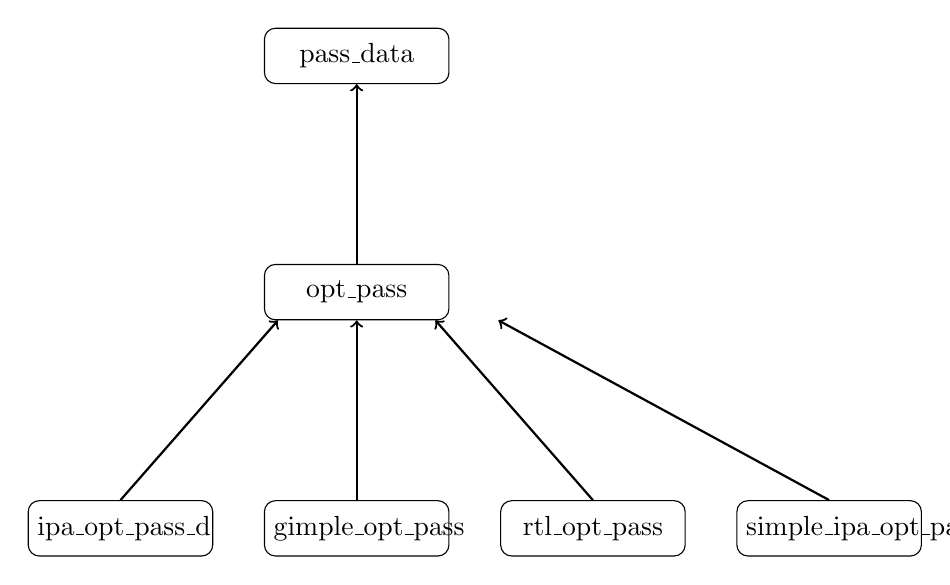
\begin{tikzpicture}[node distance = 5cm, auto]
    % Place nodes
    \node [block]                         (pass_data)   {pass\_data};
    \node [block, below of=pass_data]     (opt_pass) {opt\_pass};

    \node [block, below of=opt_pass]        (gimple_opt_pass) {gimple\_opt\_pass};
    \node [block, left of=gimple_opt_pass] (ipa_opt_pass_d)  {ipa\_opt\_pass\_d};
    \node [block, right of=gimple_opt_pass]  (rtl_opt_pass)    {rtl\_opt\_pass};
    \node [block, right of=rtl_opt_pass]    (simple_ipa_opt_pass) {simple\_ipa\_opt\_pass};

    % Draw edges
    \draw[->, thick]    (opt_pass.north)          -- (pass_data.south);

    \draw[->, thick]    (gimple_opt_pass.north)      -- (opt_pass.south);
    \draw[->, thick]    (ipa_opt_pass_d.north)       -- ([xshift=-1cm]opt_pass.south);
    \draw[->, thick]    (rtl_opt_pass.north)         -- ([xshift=1cm]opt_pass.south);
    \draw[->, thick]    (simple_ipa_opt_pass.north)  -- ([xshift=1.8cm]opt_pass.south);


\end{tikzpicture}
}
\end{center}
\caption{GCC Passes Hierarchy}
\label{fig:opt_uml}
\end{figure}


\end{subsection}

%    Para realizar otimizações considerando as interações entre as rotinas,
%é utilizado um grafo de chamada de funções (\texttt{cgraphs}). Aqui as rotinas são
%representadas como um vértice no grafo, e existe um arco de $f$ à $g$
%quando há uma chamada de $g$ a partir de $f$. Dependendo da linguagem de
%programação utilizada, construir tais grafos pode ser uma tarefa simples pois
%as chamadas são especificadas estaticamente, como é o caso de Fortran; mas
%isto pode se tornar algo extremamente complexo quando orientação à objetos é
%empregada, pois é possível sobrescrever métodos.
%
%    Os grafos de chamadas de funções permitem otimizações que eliminem chamadas
%de funções, economizando assim o custo da chamada, e ainda permitem com que as
%funções sejam emitidas por ordem de proximidade, evitando com que o salto no
%fluxo de execução seja demasiado longo, o que implicaria em \textit{cache miss}.
%Também é possível propagar informações a respeito de outras funções, por exemplo
%propagar que uma certa função não altera um estado global ou interno desta
%(e.g. imprimir na tela, alterar um objeto), e em seguida calcular o resultado
%desta em tempo de compilação e remover sua chamada. Isto permite binários menores
%e código mais rápido, pois evita a necessidade de computar valores em tempo de
%execução.
%

%Um exemplo é o \textit{Register Transfer Language} (RTL) onde o código é
%representado como uma sequência de instruções em uma máquina de infinitos
%registradores. 

\begin{subsection}{GNU Toolchain and the Classical Compilation Scheme}

    A \textit{toolchain} is a set of tools that are chained together for
	developing software. Usually, a \textit{toolchain} consists of a
	compiler, an assembler, and a linker, but can also contain more tools
	such as a debugger, and even a text editor.

	GNU provides a toolset for software development called GNU Toolchain.
	Is part of this toolchain:

\begin{itemize}
    \item \textit{Binutils}, a set of tools containing the linker \textit{ld},
	the assembler \textit{as}, and other tools\footnote{\url{https://www.gnu.org/software/binutils/}}.

    \item The driver \texttt{gcc}, responsible for calling the compilers \texttt{cc1},
        \texttt{cc1plus}, \texttt{f951} for C, C++ and Fortran, respectively, and also
		responsible to interact with other tools from the toolchain.

    \item The \texttt{glibc} library.

    \item The \textit{gdb} debugger.
\end{itemize}

These tools interact with each other in the following order: first, the code in the Source
Language is compiled using GCC to a machine language, then the code is assembled using the
assembler \textit{as}, which builds an object file, and then the linker \textit{ld} will
collect all generated object files and link together
into a single binary or library. \ref{fig:gnu_toolchain} illustrates this process.
This is automatically done by the gcc driver.

\begin{figure}
\tikzstyle{block} = [rectangle, draw, fill=white,
    text width=6em, text centered, rounded corners, node distance=6.5cm, auto, minimum height=2em]
\tikzstyle{line} = [draw, -latex]
\tikzstyle{cloud} = [draw, ellipse,fill=white, node distance=2cm,
    minimum height=2em]
\begin{center}
\scalebox{0.7}{
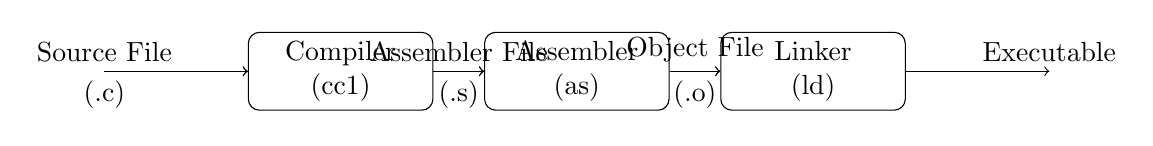
\begin{tikzpicture}[node distance = 3cm, auto]
    % Place nodes
    \node [block]                      (cc1) {Compiler \\ (cc1)};
    \node [block, right of = cc1]      (as) {Assembler\\(as)};
    \node [block, right of = as]       (ld) {Linker\\(ld)};
    \coordinate [left of=cc1]          (fonte);
    \coordinate [right of=ld]    (bin);

    % Draw edges
    \draw[->]    (cc1.east)    -- (as.west)       node[midway, above] {Assembler File};
    \draw[->]    (cc1.east)    -- (as.west)       node[midway, below] {(.s)};
    \draw[->]    (as.east)     -- (ld.west)       node[midway, above] {Object File};
    \draw[->]    (as.east)     -- (ld.west)       node[midway, below] {(.o)};
    \draw[->]    (fonte.west)  -- (cc1.west)      node[pos=0, above] {Source File};
    \draw[->]    (fonte.west)  -- (cc1.west)      node[pos=0, below] {(.c)};
    \draw[->]    (ld.east)     -- (bin.west)      node[pos=1, above] {Executable};
\end{tikzpicture}
}
\end{center}
\caption{Compilation pipeline}
\label{fig:gnu_toolchain}
\end{figure}

This process is traditionally used to compile complex software together with
some tool that controls this process for each file, such as GNU Make, as
illustrated in Figure \ref{fig:classical_build}. here, each file is compiled
individually, going through every compilation process (generation of assembler,
then encapsulated into an object file), then every file is linked together with
\textit{ld}. In GNU Make, it is possible to explicitly determine the
dependencies of each file, the compilation can be done in parallel between
files that do not depend on each other.

%Esse processo é tradicionalmente usado para compilar \textit{softwares} complexos,
%em conjunto com uma ferramenta que controla a geração de arquivos objetos e executáveis
%como o GNU Make, como ilustrado na Figura \ref{fig:classical_build}. Aqui cada arquivo
%é compilado individualmente, passando por todos os processos da compilação (tradução
%para a linguagem intermediária, otimização, tradução para a Linguagem Alvo,
%e encapsulamento no arquivo objeto), para que em seguida eles sejam ligados por um
%linkeditor como o LD. Através do Make, onde é possível explicitar as dependências de
%um arquivo, a compilação pode ser efeutada em paralelo entre arquivos que não dependem
%uns dos outros.

In this process, it is not possible to apply optimizations observing the
program as a whole, because the compiler has no information about the
information present on functions that are outside its Translation Unit (TU). A
Translation Unit is the content of the file which will be translated into
another language (\textit{e.g.} the content of a .c file plus all headers it
inclues) Therefore, every optimization are applied only local to its TU.

%Neste processo, não é possível aplicar otimizações observando o programa como
%um todo, pois o compilador não tem informações sobre as funções que estão em
%outros arquivos. Sendo assim, todas as otimizações são aplicadas localmente
%usando apenas o contexto do arquivo.

\begin{figure}
\tikzstyle{block} = [rectangle, draw, fill=white,
    text width=6em, text centered, rounded corners, node distance=3cm, auto, minimum height=2em]
\tikzstyle{line} = [draw, -latex]
\tikzstyle{cloud} = [draw, ellipse,fill=white, node distance=2cm,
    minimum height=2em]
\begin{center}
\scalebox{0.7}{
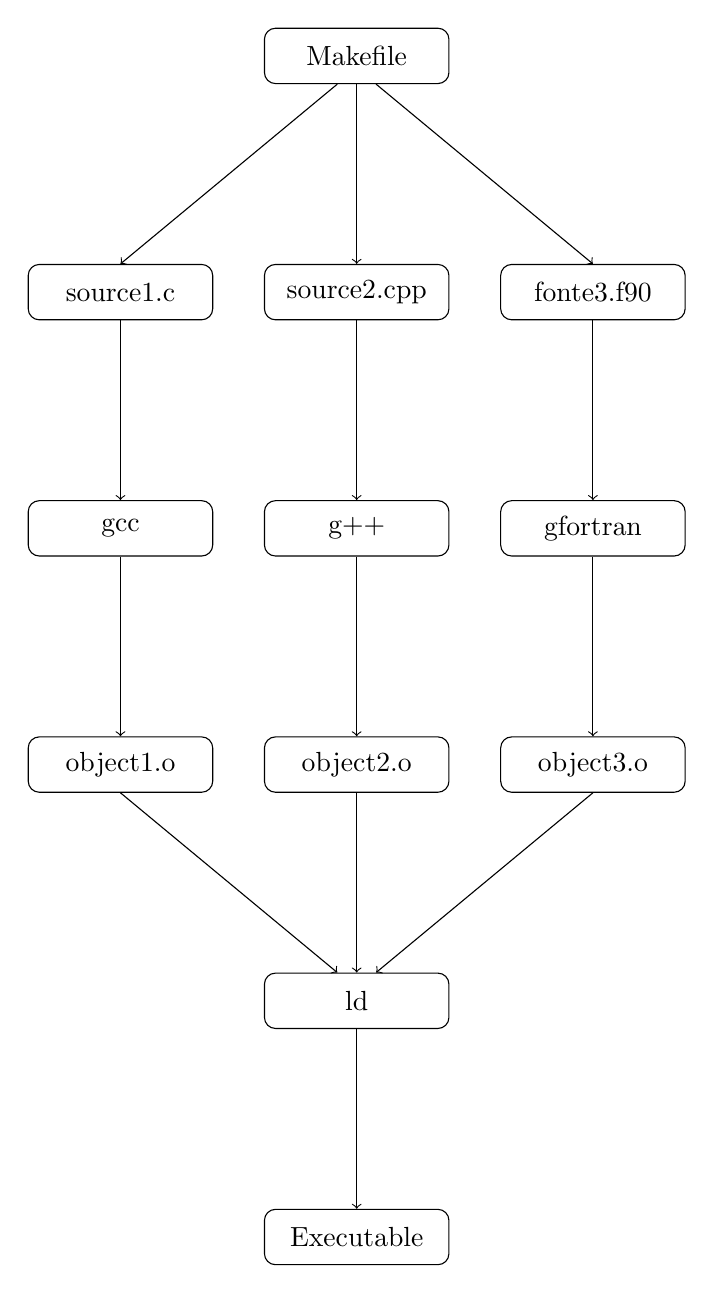
\begin{tikzpicture}[node distance = 3cm, auto]
    % Place nodes
    \node [block]                         (make)   {Makefile};
    \coordinate[below of=make]            (c);
    \node [block, left of=c]              (fonte1) {source1.c};
    \node [block, right of=fonte1]        (fonte2) {source2.cpp};
    \node [block, right of=fonte2]        (fonte3) {fonte3.f90};

    \node [block, below of=fonte1]        (gcc)      {gcc};
    \node [block, below of=fonte2]        (g++)      {g++};
    \node [block, below of=fonte3]        (gfortran) {gfortran};

    \node [block, below of=gcc]           (objeto1) {object1.o};
    \node [block, below of=g++]           (objeto2) {object2.o};
    \node [block, below of=gfortran]      (objeto3) {object3.o};

    \node [block, below of=objeto2]       (ld) {ld};

    \node [block, below of=ld]            (bin) {Executable};

    % Draw edges
    \draw[->]    ([xshift=-0.7em] make.south)   -- (fonte1.north);
    \draw[->]    (make.south)   -- (fonte2.north);
    \draw[->]    ([xshift=+0.7em] make.south)   -- (fonte3.north);

    \draw[->]    (fonte1.south)   -- (gcc.north);
    \draw[->]    (fonte2.south)   -- (g++.north);
    \draw[->]    (fonte3.south)   -- (gfortran.north);

    \draw[->]    (gcc.south)   -- (objeto1.north);
    \draw[->]    (g++.south)   -- (objeto2.north);
    \draw[->]    (gfortran.south)   -- (objeto3.north);

    \draw[->]    (objeto1.south)   -- ([xshift=-0.7em]ld.north);
    \draw[->]    (objeto2.south)   -- (ld.north);
    \draw[->]    (objeto3.south)   -- ([xshift=+0.7em]ld.north);

    \draw[->]    (ld.south)   -- (bin.north);


\end{tikzpicture}
}
\end{center}
\caption{Classic compilation scheme of a program.}
\label{fig:classical_build}
\end{figure}

\end{subsection}

\begin{section}{Contributing to GCC}\label{sec:contributing}

GCC is a free software program, and its development is often done by
contributors worldwide, paid or not. As with every Free Software project,
the contribution must be sent in a specific manner and fulfill a list
of attributes to ensure the quality of the contribution.

\begin{subsection}{Cloning GCC}

Since 2020, GCC switched its main software versioning system from Subversion
to Git \citep{gcc_git}. In order to work on GCC, you must create a working
copy of the latest revision of GCC, which can be archived by \textit{cloning}
the GCC repository. Assuming you have git installed, you can clone
gcc by

$$\texttt{\$ git clone git://gcc.gnu.org/git/gcc.git gcc\_git\_gnu}$$

This will create a folder called ``gcc\_git\_gnu'' in your working directory.

\end{subsection}

\begin{subsection}{Compiling GCC}

GCC is written in C++11, and therefore you need a working C++11 compiler to
compile it. It can be an old version of GCC itself distributed by your Linux
distro such as GCC 4.9, or even other compilers such as \textit{clang}. The
additional packages are also required:
\begin{itemize}
	\item Flex.
	\item Bison.
	\item GNU Multiprecision Library (GMP).
	\item GNU MPFR Library.
	\item GNU MPC.
	\item Libzstd Compression Library.
\end{itemize}

GCC supports several compilation modes by adding new flags into the
\texttt{configure} script. The main ones for development are:
\begin{itemize}

	\item \texttt{-{}-disable-bootstrap}: disable a feature called
	\textit{bootstrap}, which makes the compiler compile itself several times to
	remove any vestige of the system compiler being used. This reduces the time
	taken to compile the project.

	\item \texttt{-{}-enable-checking=release}: disable most sanity checkings
	in the compiler. This is useful for testing the compiler performance or to
	build a compiler that may be used in production.

	\item \texttt{-{}-disable-multilib}: disable support for 32-bit x86 binaries on
	amd64 machines. This requires additional packages in your system that you may
	not want to install.

	\item \texttt{-{}-enable-languages=c,c++}: compiles only C and C++ compilers,
	avoid generating other compilers that may be useless in your development
	process.
\end{itemize}

To compile GCC, you must \textbf{make sure to never compile in a directory inside the
gcc project}, otherwise you will contaminate your repository with temporary files.
In our case, you should not compile it in any folder under the
\texttt{gcc\_git\_gnu} folder.


Given that your current shell is in \texttt{gcc\_git\_gnu} folder, use
\texttt{cd ..} to return to a previous folder, create a new directory
\texttt{build}, enter it using \texttt{cd build} and then run:

\begin{align}
\texttt{\$ ../gcc\_git\_gnu/configure} & \texttt{ -{}-disable-bootstrap -{}-disable-multilib} \nonumber \\
& \texttt{ -{}-enable-languages=c,c++} \nonumber
\end{align}
Then finally:
$$\texttt{\$ make -j<num\_jobs>}$$
where \texttt{<num\_jobs>} are the number of cores available in your computer.

If there is a missing library in your system, the build process will notice
you. In this case, you should install it to proceed the compilation.
\end{subsection}

\begin{subsection}{Installing and Testing GCC}
One quick test that can be made to check if your modifications are indeed
working is to install the compiler and try to compile some toy programs.
To install GCC in a custom folder (for instance, in \texttt{/tmp}) you
should install using an additional parameter \texttt{DESTDIR}. For instance,
if you want to install GCC on \texttt{/tmp/gcc\_trunk}, you should run:
$$\texttt{\$ make DESTDIR=/tmp/gcc\_trunk install}$$

Once installed, you can launch the new version of gcc simply by pointing
the binary in the shell:
$$\texttt{\$ /tmp/gcc\_trunk/usr/local/bin/gcc --version}$$
If it shows the current version you compiled, then probably everything is
correct. Compile some toy programs to check if the compiler is indeed working.

When modifying the GCC code, you must always check if you broke something
that is already working, however, since you cloned a development branch,
it is possible that \textit{something was already broken} in the upstream
itself, and when you
run the testsuite, you may think that you broke something when in fact
you did not. Therefore, you should run the testsuite before and after your
development, and take down notes about the tests in which are failing.

You can run the extensive GCC testsuite by launching make as:
$$\texttt{\$ make check-gcc -j<num\_cores>}$$
Sometimes, you just want to launch a single testsuite, for instance,
the \texttt{dg.exp}. In this case, you can launch make with:
$$\texttt{\$ make check-gcc -j<num\_cores> RUNTESTFLAGS='dg.exp'}$$
or even run a single test of a suite, for instance:
$$\texttt{\$ make check-gcc RUNTESTFLAGS='dg.exp sinatan-1.c'}$$

However,  a good test is to check if \textit{bootstrap} is working after your
changes. This will make the compiler compile itself several times with various
optimizations levels to ensure that everything is working. In this case, just
create a new directory \texttt{build\_bootstrap} and proceed by:

\begin{align}
\texttt{\$ ../gcc\_git\_gnu/configure} & \texttt{ -{}-disable-multilib} \nonumber \\
& \texttt{ -{}-enable-languages=c,c++} \nonumber
\end{align}


\end{subsection}

\begin{subsection}{Debugging GCC}

Sometimes, finding the problem in your changes is not trivial at all. If you
are familiar with \textit{gdb}, you can launch GCC under it for finding the
problems.

There are two cases, requiring a distinct approach. One if you want to
\textit{debug the compiler (cc1)} or if you want to \textit{debug the driver}.
in the first case, you should launch the compiler with

	$$\texttt{\$ /tmp/}\cdots \texttt{/gcc -wrapper gdb,args file.c}$$
	in the later
	$$\texttt{\$ gdb /tmp/}\cdots \texttt{/gcc -args file.c}$$
	such difference comes from the fact that the \textit{driver} is responsible
	to call the correct compiler, and this wrapper will simply make things
	easy for the user by instructing the driver to call the compiler under gdb.
	When debugging the driver, there is no need for calling the wrapper at all,
	since the binary is already exposed to the user.


We will not enter in details about how to use gdb here, but
\cite{stallman1988debugging} provide a walkthrough about how to use it.

\end{subsection}

\begin{subsection}{Writing and Sending Patches}

Writing patches are quite straightforward. First, be aware that GCC uses the
GNU Coding Style, and therefore your text editor must be configured
accordingly. In the \texttt{contrib} folder, there are some configuration files
for Vim, which you should be using if you code using such text editor.

But perhaps one of the most bureaucratic steps in Free Software development is
sending the changes back to the community for review. However, once you master
this process, sending changes comes naturally and can be done quite fast.

First, create a new branch for you to work on. A quick way of doing this is
by $$\texttt{\$ git checkout -b feature}$$ This will create a new branch
\textit{feature}, and now you are ready to implement your changes. Once you
have tested, you should \textit{commit} then. This can be done with the
sequence of commands
\begin{align}
\texttt{\$ } & \texttt{git add .} \nonumber \\
\texttt{\$ } & \texttt{git commit -v \nonumber}
\end{align}
then text editor window will show up for you to explain what this
commit does. Commits have a title that should not have more than
60 characters (but they can depending on the situation),
followed by a more detailed text, and the
ChangeLog. For examples of how you should write a commit,
run $\texttt{\$ git log}$ to show the most recent commits. For an example
about how to create a detailed changelog, read the file
\texttt{gcc/ChangeLog}. Do not underestimate this task, try to
write a good commit message because people will review it.
If your patch contains a new feature (for instance, a match and
replace optimization), you should \textbf{write a test for it} as
well.

Once committed, you should switch back to the \textit{master} branch
and update it using
\begin{align}
\texttt{\$ } & \texttt{git checkout master} \nonumber \\
\texttt{\$ } & \texttt{git pull \nonumber}
\end{align}
	because probably between your changes, someone already commited a new
	patch. Now you should put place your commit (which is in \textit{feature})
	on top of \textit{master} by
	$$\texttt{\$ git rebase master feature}$$
	now if you run \texttt{git log}, you should see your commit on the top.
	Now generate a patch by
	$$\texttt{\$ git format-patch HEAD\textasciitilde1 -o /tmp/}$$
	which will generate a file in \texttt{/tmp/} folder.

	Once the patch file is ready, use \texttt{contrib/check\_GNU\_style.py}
	script on your patch to find if it respects the GNU codestyle. If
	everything is correct, then you can send the patch using
\begin{align}
\texttt{\$ git send-email} & \texttt{ -{}-annotate  -{}-to='gcc-patches@gcc.gnu.org'} \nonumber \\
& \texttt{ file.patch \nonumber}
\end{align}
	however, you might need to configure \texttt{git send-email} before you can use it
	\citep{flusp_tavares}.

\end{subsection}

\begin{subsection}{Where to Begin}
	Finding where to start contributing is not trivial. There are several
	files to look on, and no clear signal of problem anywhere. However,
	a good start is:
	\begin{itemize}
		\item Check if you can come with a new \texttt{match.pd} rule. This
		is how we started contributing to the compiler \citep{sinatan_flusp}.

		\item GCC was originally written in C, then switched to C++. Most
		Intraprocedural passes are still written in plain C and would be
		very interesting to see them encapsulated into a class

		\item Read the EasyHacks page\footnote{https://gcc.gnu.org/wiki/EasyHacks}.
	\end{itemize}

	You can also subscribe to the \texttt{gcc@gcc.gnu.org} mailing list for help,
	just make sure to send e-mails in plain-text mode, otherwise it will be
	classified as spam.

\end{subsection}

\end{section}

\end{section}

\begin{section}{Parallel Computing}\label{sec:parallel_computing}
\label{sec:parallel_comp}

Parallel Computing is the act of coordinating several executions flow operating
simultaneously in one or more computers to archive some common objective. It
became a tendency in contemporary computing due to affordability and reduced
production cost of multicore and manycore processors when compared to a
single-core, sequential processor of the same computational power.


%    A Computação Paralela é o ato de coordenar vários fluxos de
%execução operando simultaneamente em um ou mais computadores para
%atingir um objetivo em comum. Ela se tornou uma tendência na
%computação contemporânea por conta da facilidade de aquisição
%e custo de produção reduzido dos processadores \textit{multicore}
%e \textit{manycore}, em relação a um processador de igual desempenho
%com apenas um núcleo.

To illustrate this evolution in multicore processors, \cite{42years}
published a figure showing the number of transistors, cores, and
performance of each core since 1970, as presented in Figure
\ref{fig:42years}. We can see in this figure that Moore's law
is still true, however, the sequential performance of the processors
is slowing down, while the number of cores grows exponentially
since 2008. This justifies the use of parallel computing when possible
for the maximum usage of computational resources available.

%    Para ilustrar a evolução dos processadores \textit{multicore}, \cite{42years}
%    publicou um gráfico mostrando o número
%de transistores, núcleos e desempenho de cada núcleo desde 1970,
%apresentado na Figura \ref{fig:42years}.
%Neste gráfico é possível notar que a Lei de Moore ainda se aplica,
%mas a desempenho sequencial dos processadores está em desaceleração,
%enquanto o número de núcleos cresce exponencialmente desde 2008. Isto
%justifica o uso de computação paralela sempre que possível para que
%seja utilizado o máximo dos recursos computacionais disponíveis.

In this section, we discuss some basic concepts about parallel computing,
and some algorithms which are useful when parallelizing a program.

%    Nessa seção são discutidas alguns conceitos básicos de computação
%paralela e alguns algoritmos úteis na paralelização de programas.

\begin{figure}[ht]
 \centering
 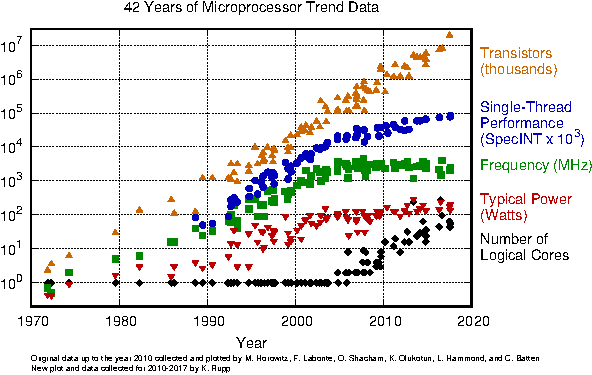
\includegraphics[scale=1.5]{42-years-processor-trend.pdf}
 \caption{42 years of microprocessor trend data \citep{42years}.}
 \label{fig:42years}
\end{figure}

\begin{subsection}{\textit{Speedup}}
	One way to measure the time reduction of a parallel implementation
	is through the concept of speedup. 

\begin{definition}
	Let $T_1$ be the time of a sequential algorithm and $T_n$ the time
	of this same algorithm parallelized with $n$ cores. Then the
	\textbf{speedup} $S_n$ is given by:
    $$ S_n = \frac{T_1}{T_n} $$
\end{definition}

%    Uma maneira de medir o ganho de tempo em uma implementação paralela
%de um algoritmo é através no conceito de \textit{speedup}. Sejam $T_1$
%o tempo do algoritmo sequencial e $T_n$ o tempo desse algoritmo paralelizado
%    com $n$ núcleos de processamento. Então o \textit{speedup} $S_n$
%é dado por:

\end{subsection}


\begin{subsection}{Flynn Taxonomy}
%	Mesmo com a evolução dos processadores \textit{multicore} e
%\textit{manycore}, estas não são as únicas arquiteturas disponíveis para
%realizar computação paralela. Michael J. Flynn \citep{pacheco:2011} definiu
%uma taxonomia das arquiteturas, mas vale destaque para duas delas:

Even with the evolution of multicore and manycore processors, those are not the
only architectures available for parallel computing.  Michael J. Flynn
\citep{pacheco:2011} defined a taxonomy of architectures, however, two of them
must be highlighted:

\begin{enumerate}
	\item \textbf{SIMD} - \textit{Single Instruction, Multiple Data}. Those are
	vectorial processors that allow a single operation to be executed
	simultaneously in every element of a vector. Some examples are the Intel SSE
	instruction set, and also the \textit{Graphics Processing Units} (GPU) although
	this last one is not considered a pure SIMD architecture.

    \item \textbf{MIMD} - \textit{Multiple Instruction, Multiple Data}. Those
are the completely independent multicore systems, capable of
executing tasks asynchronously. Here we find both shared memory and distributed memory architectures.

\end{enumerate}
\end{subsection}

\begin{subsection}{Parallel Programming in Shared Memory}
	One way of doing Parallel Computing is through a shared memory
	behind the cores or processors. Here, a shared memory is connected
	through a bus to all processors, allowing read and write of data.
	To avoid concurrency problems, both locking and synchronization mechanisms
	are required.

%	Uma maneira de permitir Computação Paralela é através de
%uma memória compartilhada. Aqui vários processadores ou núcleos
%são ligados através de um barramento a uma memória compartilhada entre
%todos os processadores, que permite leitura e escrita de dados.
%Para evitar problemas de concorrência, são necessários mecanismos de
%travas e sincronização.

	Here, most resources are provided by the Operating System (OS),
	and therefore a brief explanation is required about its abstractions.

%	 Aqui, muitos dos recursos para sincronização são fornecidos pelo
%Sistema Operacional (OS), e portanto é necessário explicar um pouco
%das abstrações que ele fornece.

\begin{subsubsection}{Process and Threads}

	Before the existence of multicore processors, a processor
	could only execute a program at a time. With this fact in
	mind, Operating System developers created a series of abstractions
	so that the user could have the illusion that several programs were
	executing simultaneously. Although this is not true anymore, this
	is the primary fact between the concept of Process and Threads.

%	Antigamente, os processadores eram capazes de executar apenas
%um programa por vez. Com isto em mente, os desenvolvedores
%de Sistemas Operacionais criaram uma série de abstrações para que fosse
%possível dar a ilusão ao usuário que vários programas estavam executando
%ao mesmo tempo. Embora isso não seja mais um fato, já que hoje os processadores
%são capazes de executar vários fluxos de execução simultaneamente, essa
%é a principal motivação do conceito de Processos e \textit{Threads}.

A \textit{process} is an abstraction provided by the Operating System which
gives to the program the illusion that it has the processor's monopoly
\citep{love:2005}. Each process has its own memory region, and sharing
information between processes must be done through Interprocess Communication
(IPC). One example of such is the \texttt{shmget} call, from \texttt{System V},
in which Linux still supports \citep{shmget}, or through a Pipe \citep{pipe}.

%	Um \textit{Processo} é um modelo de abstração do Sistema Operacional que
%dá a um programa a ilusão de que ele tem o monopólio do processador
%\citep{love:2005}. Cada processo tem a sua região de memória privada por
%padrão, e para que processos possam compartilhar memória, isso deve ser 
%explicitado no programa. Um exemplo onde isso pode ser feito é através das
%chamadas \texttt{shmget} do extinto \texttt{System V}, mas cujo o Linux ainda
%oferece suporte \citep{shmget}.

Each process contains at least one execution flow, and each execution
flow is called a \textit{thread}. Each thread inside a process
shares memory with every other thread from the same process, except
for its stack and the Thread Local Storage (TLS) region, which turns
the development of communication mechanisms easier.

When parallelizing a program, the programmer must choose between using threads
or processes. By selecting threads, the programmer will have the advantage of
having access to global data structures and therefore an easy communication
between the threads. However, race conditions must be solved individually,
which may become cumbersome when the software is really large. By selecting to
parallelize through processes, most race conditions may fade away, but then the
issue revolves around find \textit{what} must be shared and how to do an
efficient communication between processes, as IPC can be slow.

Unix processes are created through a system call named \textit{fork}. On
Linux, forking will clone the current process into another, and copy
the pages only when modified, a process named Copy on Write (CoW). This
may turn into an additional overhead when processes are chosen instead
of threads \citep{abbas_cow}.

%Cada processo contém pelo menos um fluxo de execução, e cada fluxo de
%execução é chamado de \textit{thread}. Cada \textit{thread} dentro
%de um processo compartilha memória com as demais \textit{threads}
%do processo, facilitando assim o desenvolvimento de mecanismos de
%comunicação através de uma memória compartilhada.

\end{subsubsection}

\begin{subsubsection}{Sincronization Mechanisms}

An Operating System usually provides synchronization mechanisms to control
several threads of a process or even several processes. These mechanisms are
often implemented with the help of hardware resources, however, they can also
be implemented purely in software.

%	Seja através de auxílio do \textit{hardware}, ou com algoritmos
%puramente implementados em \textit{software}, o Sistema Operacional
%costuma fornecer mecanismos de sincronização para coordenar as várias
%\textit{threads} de um processo, ou até mesmo vários processos.

One of such mechanisms are \textit{Semaphores} \citep{dijkstra1965}.  A
semaphore is a counter which can assume non-negative integer values with
two atomic operations: \texttt{P} to decrement it, or \texttt{V} to
increment it. When the semaphore reaches 0, the next thread that will try
to decrement it will be blocked. Its execution will only be resumed when
another thread increments the semaphore.

%\citep{dijkstra1965}. Um semáforo nada mais é que um contador que assume
%valores não negativos com duas operações atômicas: \texttt{P} para
%decrementá-lo, e \texttt{V} para incrementá-lo. Quando o semáforo atinge o
%valor 0, a \textit{thread} que em sequência tentar decrementá-lo será bloqueada. A
%sua execução apenas será retomada quando o semáforo for novamente incrementado
%por outra \textit{thread} \citep{semaphore}.

Semaphores can also be used to solve the critical section problem, which is
when only one thread must be executing a section of the code at a time.
However, such a problem is often solved using \textit{mutexes}.

%    Semáforos também podem ser utilizados para resolver o problema da
%seção crítica, que é uma seção de código que apenas uma \textit{thread}
%deve poder executar por vez, embora seja mais comum a utilização
%de \textit{Mutexes}.

Mutexes are a structure that ensures the mutual exclusion of a code region, as
illustrated in Figure \ref{fig:mutex}. In this figure, three threads are
started executing a function named $f$, but only one can execute the critical
section at the time.

%\textit{Mutexes} nada mais são que uma estrutura que garante a exclusão
%mútua de uma região, conforme ilustrado na Figura \ref{fig:mutex}. Nessa
%figura, três \textit{threads} são iniciadas executando a função $f$, mas
%apenas uma pode executar a seção crítica.

When a mutex is locked, every other thread that tries to access
the critical section will be blocked by the Operating System,
ensuring that only one thread will be executing this section.
Every blocked thread will be unlocked when the thread that
locked the mutex unlocks it. This is the main difference between
a mutex and a binary semaphore.

%    Quando o \textit{mutex} \texttt{lock} é travado,
%todas as outras \textit{threads} que tentarem acessar a seção crítica
%serão bloqueadas pelo Sistema Operacional, garantindo assim que apenas
%uma \textit{thread} esteja executando a seção crítica.
%As \textit{threads} bloqueadas somente voltarão a executar quando o
%    \textit{mutex} for desbloqueado pela \textit{thread} que o travou.
\begin{figure}
      \begin{lstlisting}[
        language=pseudocode,
        style=pseudocode,
        style=wider,
        functions={},
        specialidentifiers={extern, call, async, mutex_t},
      ]
        extern function mutex_lock, mutex_unlock;
        mutex_t lock;

        async function f()
            mutex_lock(lock);
                // Critical section
            mutex_unlock(lock);
        end

        function main()
            for i=1, 3 do
                call f;
            done
        end
      \end{lstlisting}
      \caption{A mutex usage illustration.}
      \label{fig:mutex}
\end{figure}

Another useful synchronization mechanism is the barriers. A barrier is a point
in the program where once a thread executes it, it will be blocked until every
other thread reach the same point, as illustrated in Figure \ref{fig:barrier}.
This is very useful to avoid that one thread advances in the execution of a
code when it should be waiting for the result of some computation by another
thread. Barriers also receive an integer specifying how many threads should
reach the barrier for every thread to be allowed to continue with its
execution.

%Outro mecanismo de sincronização muito útil são as Barreiras. Uma barreira
%é um ponto no programa onde, assim que a \textit{thread} o executar, ela
%será bloqueada até que todas as \textit{threads} cheguem ao mesmo ponto, como
%ilustrado na Figura \ref{fig:barrier}.
%Isso é bastante útil para evitar que uma \textit{thread} avance na execução
%do código enquanto ela deveria estar aguardando o resultado da computação
%de outras \textit{threads}. As barrerias também costumam receber um parâmetro
%de inicialização indicando quantas \textit{threads} precisam atingir a
%barreira para que todas as \textit{threads} que a atingiu sejam desbloqueadas.

\begin{figure}[ht]
 \centering
 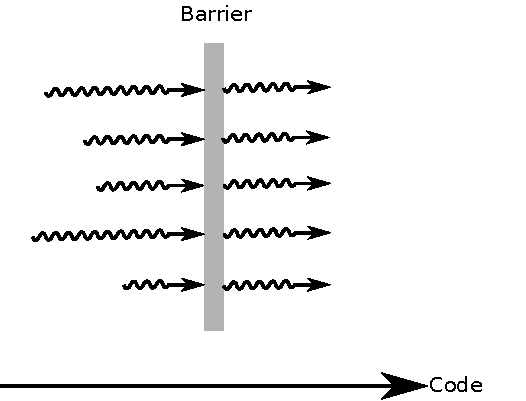
\includegraphics[scale=1.0]{barrier.pdf}
 \caption{A barrier usage illustration.}
 \label{fig:barrier}
\end{figure}

Except for semaphores, every mechanism mentioned above is implemented in the
\textit{pthread} library. Semaphores, on the other hand, are available in Linux
through the \texttt{semaphore.h} interface.

%Por fim, exceto os semáforos, todos esses mecanismos mencionados acima são
%implementados na biblioteca \texttt{Pthread}. Já os semáforos estão disponíveis
%no Linux através da interface \texttt{semaphore.h}.

\end{subsubsection}

\begin{section}{Power and Energy}\label{sec:power}

When we want to measure how much energy a computer is consuming, there are
sensors to measure the \textit{Instantaneous Power}. However, power $P$ is
defined as the time rate of energy transferred \citep{young2006sears}.
Therefore, to compute energy measuring the power consumption of a system: $$P =
\frac{dE}{dt} \quad \Rightarrow \quad E = \int_{0}^{t'} P(t)dt$$ where $t'$ is
the elapsed time of the experiment. However, we can only measure information of
the sensor in discrete time, and not continuously.  Therefore we can
approximate this integral by using two Riemann sums.

Assume that we collected $n$ measurements of the sensor at times
$t_1, t_2, \cdots, t_n$ with a distance of $\Delta t$ from each other.
Now, given two measured points at time
$t_i$ and $t_{i+1}$, we define a \textit{minimum} and \textit{maximum} $m_i$ and $M_i$
such that:
$$m_i = \min\{P(t_i), P(t_{i+1})\} \quad \text{ and } \quad M_i = \max\{P(t_i), P(t_{i+1})\}$$
Then, assuming that for every $x \in [t_i, t_{i+1}]$ we have
$$m_i \leq P(x) \leq M_i$$
this means that:
$$\sum_{i=1}^{n-1} m_i\Delta t \leq E \leq \sum_{i=1}^{n-1} M_i\Delta t$$
Which can give us a way to measure the \textit{error} of our integration
process just by computing $\sum_{i=1}^{n-1} M_i\Delta t -
\sum_{i=1}^{n-1} m_i\Delta t = \epsilon$. This can also capture the error of the sensor
itself by representing the real value as between a range of two values, and
the lower bound on $m_i$ and the upper bound in $M_i$.

\end{section}

%\begin{subsubsection}{O Problema do Produtor-Consumidor}
%    Uma estrutura de dados muito útil em computação paralela
%é uma fila completamente \textit{Thread-safe}, ou seja,
%que várias \textit{threads} possam inserir e remover dados dessa
%fila simultaneamente sem o risco de perda de dados. Essa fila
%pode ser usada na comunicação entre as \textit{threads}, por
%exemplo: uma insere trabalho na fila, outra retira trabalho da
%fila. Isso permite com que \textit{pipelines}, ou escalonamento
%dinâmico de trabalho sejam implementados.
%
%Para implementar essa fila, são necessários dois semáforos e um
%\textit{mutex}. Um semáforo deve ser inicializado com o tamanho máximo
%da fila, e na inserção de um dado, esse semáforo deve ser decrementado
%para que, quando a fila estiver cheia, as \textit{threads} que tentarem
%inserir nela sejam bloqueadas. O outro semáforo deve ser iniciado com
%0, indicando que a fila está vazia, e incrementado quando um item for
%inserido na fila. Esse semáforo tem a finalidade de
%bloquear as \textit{threads} que tentarem remover elementos dessa
%fila quando ela estiver vazia. Assim que dados forem inseridos ou removidos
%da fila, as \textit{threads} são devidamente ``despertadas''. Isso evita gasto
%desnecessário de ciclos de processamento por não utilizar uma técnica
%chamada \textit{espera ocupada}. Por fim, um \textit{Mutex} deve ser
%utilizado para evitar problemas de concorrência ao incrementar e
%decrementar os apontadores de inicio e fim da fila.
%Uma implementação
%é apresentada na Figura \ref{fig:prod_consumer}.
%\begin{figure}
%      \begin{lstlisting}[
%        language=pseudocode,
%        style=pseudocode,
%        style=wider,
%        functions={},
%        specialidentifiers={extern, call, async, int, class, mod, semaphore_t, mutex_t},
%      ]
%        class Fifo
%            int buffer[];
%            int size;
%            int head, tail;
%            semaphore_t full, empty;
%            mutex_t lock
%
%            function init(n)
%                buffer = allocate_memory(n);
%                head, tail = 0;
%                sem_init(empty, n);
%                sem_init(full, 0);
%                mutex_init(lock);
%                size = n;
%            end
%
%            function push(element)
%                sem_p(empty);
%                mutex_lock(lock);
%                buffer[head] = element;
%                head = head + 1 mod size;
%                mutex_unlock(lock);
%                sem_v(full);
%            end
%
%            function pop()
%                sem_p(full);
%                mutex_lock(lock);
%                ret = buffer[tail];
%                tail = tail + 1 mod size;
%                mutex_unlock(lock);
%                sem_v(empty)
%
%                return ret;
%            end
%        end 
%
%      \end{lstlisting}
%      \caption{Uma implementação do Produtor-Consumidor.}
%      \label{fig:prod_consumer}
%\end{figure}
%
%\end{subsubsection}

\end{subsection}

\end{section}

% Vamos definir alguns comandos auxiliares para facilitar.

% "textbackslash" é muito comprido.
\newcommand{\sla}{\textbackslash}

% Vamos escrever comandos (como "make" ou "itemize") com formatação especial.
\newcommand{\cmd}[1]{\textsf{#1}}

% Idem para packages; aqui estamos usando a mesma formatação de \cmd,
% mas poderíamos escolher outra.
\newcommand{\pkg}[1]{\textsf{#1}}

% A maioria dos comandos LaTeX começa com "\"; vamos criar um
% comando que já coloca essa barra e formata com "\cmd".
\newcommand{\ltxcmd}[1]{\cmd{\sla{}#1}}

\chapter{Trabalhos Relacionados}
\label{chap:related_works}

Nesta seção é discutido trabalhos relacionados a paralelização de compiladores.
É importante mencionar que boa parte das pesquisa relacionada a paralelismo
em compiladores é destinada a compiladores que paralelizam. Há basicamente
duas áreas de estudo relacionadas a paralelização de compiladores, são
elas: análise de texto em paralelo, e análise de fluxo de dados em paralelo.
Estes trabalhos também são abordados nessa seção, em ordem cronológica.

Dos algoritmos apresentados na Seção \ref{chap:fundamentacao}, o algoritmo
Recursivo Descendente é o mais simples deles. \cite{Lincoln:1970:PPT:987475.987478}
propôs uma maneira de paralelizar a análise léxica de um compilador
Fortran simplesmente quebrando o código fonte em partes, mapeando as
informações de final de
linha e a posição de cada caractere, e realizando o processamento
através de operações em APL.
Posteriormente, \cite{Krohn:1975:PAC:390015.808414} estendeu o trabalho
anterior, propondo uma maneira de realizar a análise sintática, a
tradução para a AST, e a geração
de código utilizando os registradores vetoriais do supercomputador
STAR-100. Ambos os artigos também não apresentam nenhuma
análise assintótica para os algoritmos propostos, e também não apresentam
experimentos. 

Posteriormente, \cite{Mickunas:1978:PCM:800127.804105} propôs uma
paralelização do algoritmo LR($0$). Sua ideia consiste em quebrar
arbitrariamente a entrada em vários segmentos e executar um analisador em paralelo
em cada um destes segmentos. Estes analisadores (exceto o primeiro,
que executa no inicio da entrada) são modificados na tentativa de
evitar conflitos, uma vez que modificar a ordem de inicio da análise
pode impossibilitar distinguir entre o prefixo e o sufixo de uma fase.
Quando um conflito é detectado, o analisador envia a sequência de
\textit{tokens} lido até então ao analisador à sua esquerda,
retorna ao estado inicial, e reinicia a sua análise.
No termino da análise, cada analisador envia o resultado para o analisador
a sua esquerda, acumulando o resultando no primeiro analisador.
Os autores não mostraram experimentos ou
análise assintótica do algoritmo proposto. \cite{Pennello:1978:FMA:512760.512786}
implementou essa estratégia em um compilador Pascal, mas seus experimentos foram
realizados em um computador paralelo simulado.

\cite{vandevoorde1988parallel} paralelizou o \textit{Titan C compiler}, um compilador
C escrito em Modula-2. Sua implementação utiliza um analisador léxico executando
paralelamente ao analisador sintático, e os \textit{tokens} são alimentados
através de um \textit{pipeline}. Ele também propôs uma paralelização de um
analisador sintático recursivo descendente, executando novas \textit{threads}
para cada expressão da gramática após a sequência de declarações do programa,
usando como premissa que qualquer declaração de funções do programa está no
cabeçalho do
arquivo. Essa estratégia de granularidade fina necessitou a implementação de
uma maneira de controlar o paralelismo, onde foi utilizado o conceito de
WorkCrews \citep{vandevoorde1988workcrews}, limitando o número máximo de
\textit{threads} em execução simultânea. O autor relata um ganho de 10\% no
uso do \textit{pipeline} entre o analisador léxico e sintático, e um
\textit{speedup} de até $3.1\times$ utilizando 5 processadores MicroVax II em
memória compartilhada.  Entretanto, o compilador não possui estágios de
otimização e o autor não discute como paralelizar um otimizador.

De maneira similar, \cite{wortman1992} construiu um compilador de Modula-2+
paralelo. A estratégia proposta é utilizar um analisador léxico capaz de
encontrar funções no código fonte e prosseguir com a compilação em paralelo
nesse nível, gerando uma tarefa para cada função. Para solucionar problemas
relacionados a chamada de funções e
acesso a símbolos ainda não definidos, o autor propõe o uso de
uma lógica ternária na tabela de símbolos, especificando um estado
``\textit{Doesn't know yet}'' (Ainda não visto), e propõe três estratégias para
implementar essa funcionalidade. Em seguida, o autor propõe o uso de
um número fixo de \textit{threads} trabalhadoras, e o uso de uma fila de
prioridade produtor consumidor, onde as \textit{threads} deverão retirar o trabalho.
O uso de uma fila de prioridade permite com que as funções mais longas sejam
processadas primeiro. Os experimentos conduzidos pelo autor mostraram
\textit{speedups} variando de $1.5\times$ até $6\times$ utilizando 8
processadores MicroVAX II em memória compartilhada.

Deve ser destacado que os artigos até então não abordam questões relacionadas
a otimização de código. Isso porque os compiladores até então haviam poucos
passos de otimização, o que implicava em pouco tempo necessário para fazê-la.
Mesmo assim, alguns pesquisadores dedicaram-se a estudar esses passos.
\cite{Lee1994} estudou maneiras de explorar paralelismo na análise de controle
de fluxo. Os autores argumentam que os compiladores otimizadores gastam a maior
parte do tempo realizando tais análises, principalmente nas otimizações Inter
Procedurais. A análise se concentra em algoritmos que usam o grafo de controle
de fluxo como entrada, sendo assim os autores propõem uma heurística de aglutinação
para particionar tal grafo em regiões conexas e adjacentes de tamanho não maior
que um certo inteiro $s$, já que o
problema geral é NP-difícil. Os autores experimentam sua implementação utilizando
8 processadores do computador iPSC/2 em memória distribuída, e 
relatam \textit{speedups} variando de
$2.8 \times$ até $6.5\times$. Os autores relataram que o \textit{speedup} foi
limitado pela característica dos programas no teste: os arquivos consistiam
de várias funções pequenas, o que normalmente é considerado uma boa prática de
programação. Uma outra forma de explorar o paralelismo nessas estruturas
foi proposta por \cite{kramer1994combining}.

Após estes resultados, houve um aparente hiato nas pesquisas relacionadas a
compilação em paralelo. Uma causa possível é o fato de um compilador ser
um programa muito complexo, e os processadores até então ainda serem, em sua grande
maioria, sequenciais. Uma década depois, houve uma explosão de processadores
paralelos e poder computacional como um todo, como apresentado na Seção
\ref{sec:parallel_comp}, o que levou a empresas propor soluções mais eficazes para
gerar código mais eficiente. Embora não diretamente relacionado a compiladores paralelos,
algumas estruturas propostas acabam tocando nesse tópico.

\cite{whoprgoogle} propôs uma alteração no
compilador GCC com a finalidade
de possibilitar otimizações no programa como um todo. A alteração consiste
em construir um grafo de chamadas de função em relação a todo o programa,
ao contrário do modelo clássico, em que cada módulo é compilado independentemente.
Esse processo consiste em três etapas:
\begin{enumerate}
    \item \textit{Local Generation } (LGEN). Cada função do programa é compilado
        na Linguagem Intermediária, em conjunto com o grafo de chamadas de função.
        Esse estágio pode executar em paralelo.

    \item \textit{Whole Program Analysis} (WPA). O grafo de chamadas de função global
        é construído, e é decidido quais otimizações efetuar. Essa estágio
        deve ser executado sequencialmente.

    \item \textit{Local Transformations} (LTRANS). Todas as decisões aplicadas na
        etapa 2 são implementadas localmente, e o código objeto final é gerado.
        Esse estágio pode executar em paralelo.
\end{enumerate}

A Figura \ref{fig:whopr_build} retrata este processo. Essa proposta foi implementada
no GCC \citep{glek2010optimizing} com o nome de
\textit{Link Time Optimization} (LTO). A granularidade
escolhida na etapa LGEN foi paralelismo por arquivo, já na LTRANS a granularidade
escolhida são partições do arquivo objeto, e por consequência é possível otimizar
funções de um arquivo em paralelo. Os autores testaram essa implementação com o
código fonte do Mozilla Firefox e do GCC, e relataram que o GCC construiu
binários menores e mais rápidos. Os autores relataram que esse processo tornou
o processo de autocompilação do GCC duas vezes mais lenta,
mas que também houve um ganho de 20 minutos na compilação do Firefox. Em todos os
casos relatados, os passos de otimização Intra Procedural consumiu mais tempo.
\cite{livska2014optimizing} completa a análise dessa funcionalidade.
Um dos problemas que surgem é o uso elevado de memória para carregar o grafo de
chamadas de função global, necessário na fase WPA, chega a 12Gb na compilação do
Chromium e 15Gb na compilação do Kernel Linux. A maior crítica a esse processo
era o tempo necessário para recompilar todo o programa quando uma simples alteração
era efetuada em um único arquivo, inviabilizando um desenvolvimento incremental.

\begin{figure}
\tikzstyle{block} = [rectangle, draw, fill=white,
    text width=6em, text centered, rounded corners, node distance=3cm, auto, minimum height=2em]
\tikzstyle{line} = [draw, -latex]
\tikzstyle{cloud} = [draw, ellipse,fill=white, node distance=2cm,
    minimum height=2em]
\begin{center}
\scalebox{0.7}{
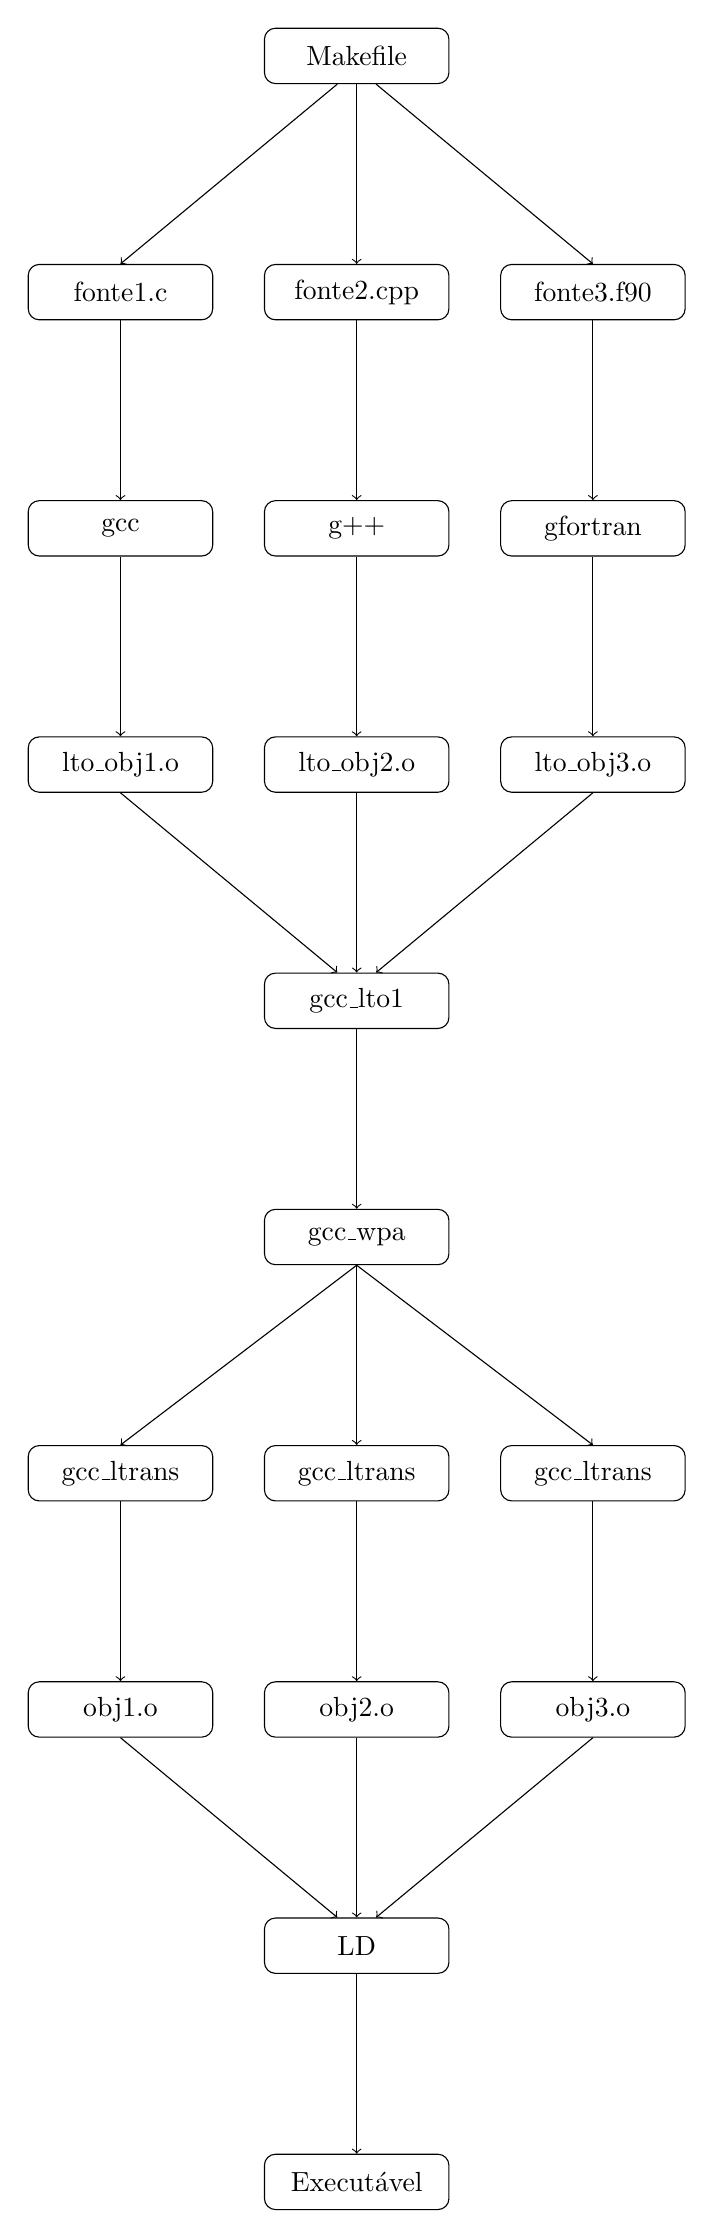
\begin{tikzpicture}[node distance = 3cm, auto]
    % Place nodes
    \node [block]                         (make)   {Makefile};
    \coordinate[below of=make]            (c);
    \node [block, left of=c]              (fonte1) {fonte1.c};
    \node [block, right of=fonte1]        (fonte2) {fonte2.cpp};
    \node [block, right of=fonte2]        (fonte3) {fonte3.f90};

    \node [block, below of=fonte1]        (gcc)      {gcc};
    \node [block, below of=fonte2]        (g++)      {g++};
    \node [block, below of=fonte3]        (gfortran) {gfortran};

    \node [block, below of=gcc]           (objeto1) {lto\_obj1.o};
    \node [block, below of=g++]           (objeto2) {lto\_obj2.o};
    \node [block, below of=gfortran]      (objeto3) {lto\_obj3.o};

    \node [block, below of=objeto2]       (gcc_lto) {gcc\_lto1};

    \node [block, below of=gcc_lto]       (gcc_wpa) {gcc\_wpa};
    \coordinate[below of=gcc_wpa]            (c2);

    \node [block, left of=c2]            (gcc_ltrans1) {gcc\_ltrans};
    \node [block, right of=gcc_ltrans1]   (gcc_ltrans2) {gcc\_ltrans};
    \node [block, right of=gcc_ltrans2]   (gcc_ltrans3) {gcc\_ltrans};

    \node [block, below of=gcc_ltrans1]   (obj1) {obj1.o};
    \node [block, below of=gcc_ltrans2]   (obj2) {obj2.o};
    \node [block, below of=gcc_ltrans3]   (obj3) {obj3.o};

    \node [block, below of=obj2]   (ld) {LD};

	\node [block, below of=ld]   (bin) {Executável};

    % Draw edges
    \draw[->]    ([xshift=-0.7em] make.south)   -- (fonte1.north);
    \draw[->]    (make.south)   -- (fonte2.north);
    \draw[->]    ([xshift=+0.7em] make.south)   -- (fonte3.north);

    \draw[->]    (fonte1.south)   -- (gcc.north);
    \draw[->]    (fonte2.south)   -- (g++.north);
    \draw[->]    (fonte3.south)   -- (gfortran.north);

    \draw[->]    (gcc.south)   -- (objeto1.north);
    \draw[->]    (g++.south)   -- (objeto2.north);
    \draw[->]    (gfortran.south)   -- (objeto3.north);

    \draw[->]    (objeto1.south)   -- ([xshift=-0.7em]gcc_lto.north);
    \draw[->]    (objeto2.south)   -- (gcc_lto.north);
    \draw[->]    (objeto3.south)   -- ([xshift=+0.7em]gcc_lto.north);

    \draw[->]    (gcc_lto.south)   -- (gcc_wpa.north);

    \draw[->]    (gcc_wpa.south)   -- (gcc_ltrans1.north);
    \draw[->]    (gcc_wpa.south)   -- (gcc_ltrans2.north);
    \draw[->]    (gcc_wpa.south)   -- (gcc_ltrans3.north);

    \draw[->]    (gcc_ltrans1.south)   -- (obj1.north);
    \draw[->]    (gcc_ltrans2.south)   -- (obj2.north);
    \draw[->]    (gcc_ltrans3.south)   -- (obj3.north);

    \draw[->]    (obj1.south)   -- ([xshift=-0.7em]ld.north);
    \draw[->]    (obj2.south)   -- (ld.north);
    \draw[->]    (obj3.south)   -- ([xshift=+0.7em]ld.north);

	\draw[->]    (ld.south)   -- (bin.north);


\end{tikzpicture}
}
\end{center}
\caption{Compilação de um programa utilizando WHOPR.}
\label{fig:whopr_build}
\end{figure}


Considerando o alto uso de memória e tempo de compilação nos casos relatados
acima, \cite{Johnson:2017:TSI:3049832.3049845} propôs o ThinLTO. A ideia é
considerar apenas parte do grafo global a cada vez, evitando carregá-lo
completamente na memória; e postergar ao máximo aplicar as otimizações possíveis,
realizando apenas análises de maneira sequencial, e aplicando-as no 
\textit{backend} em paralelo.
Os autores relataram um \textit{speedup} de até $15\times$ quando comparado a
implementação do LTO original do Clang, e até $4\times$ quando comparado a
implementação do LTO do GCC. Os autores também relataram uma diminuição considerável
no consumo de memória quando comparado ao LTO do GCC: Redução de 2.9Gb para 1Gb
na compilação do Clang, 10.8Gb para 1.0Gb no Chromium, e permitiu melhores otimizações no
\textit{Ad Delivery} da Google, enquanto a implementação do LTO no GCC
abortava a compilação após consumir mais de 25Gb de memória. O desempenho dos
binários gerados também foi similar, inclusive onde o LTO original gerava
binários mais lentos que o processo clássico de compilação. O tempo de compilação
também melhorou significativamente quando comparado ao LTO original,
mas permaneceu pior em todos os casos quando comparado ao processo clássico de
compilação.

Houve também um renascimento nas pesquisas de análise sintática em paralelo.
\cite{Barenghi:2015:PPM:2839536.2840146} encontrou uma maneira de explorar
a propriedade de Análise Local em Gramáticas com Precedência de Operadores.
Isso permitiu a construção de um gerador de analisadores sintáticos
PAPAGENO (\textit{Parallel Parser Generator}). Para isto, a gramática a
ser utilizada nesse analisador precisa ser convertida para uma Gramática
com Precedência de Operadores, conforme discutido e exemplificado pelos
autores. Testes empíricos foram efetuados implementando um analisador
JSON e outro analisador para a linguagem Lua. Em um Opteron 8378 (16 núcleos),
os autores atingiram um \textit{speedup} de até $5.3\times$ no análisador JSON
em arquivos grandes, e pouco mais de $4\times$ no analisador Lua. O algoritmo
paralelo foi comparado com os gerados pelo analisador sintático \textit{Bison},
que apenas gera código sequencial.



\chapter{Proposta de Trabalho}
\label{chap:proposta}

Neste capítulo é apresentado um plano de trabalho que será elaborado
durante o período após a qualificação, e resultados esperados.
Este trabalho tem o objetivo de trazer duas contribuições:
\begin{enumerate}
    \item Uma opção no compilador GCC para que ele seja
capaz de compilar um único arquivo em paralelo sem utilizar a
estrutura do LTO. Isso é útil para desenvolvedores que trabalham
com grandes softwares iterativamente, pois deve minimizar
gargalos gerados por arquivos grandes e cobrir os casos onde o LTO gera
binário menos eficientes que o processo clássico de compilação, fornecendo assim
uma alternativa ao LTO.
Essa tese se concentra em paralelizar os passos de otimização Intra Procedural
a nível de funções, ou seja, duas análises executarão em paralelo em funções
distintas, evitando adentrar em paralelizar a análise de fluxo de dados.

    \item Uma revisão sobre o que pode ser feito para acelerar o
processo clássico de compilação em máquinas \textit{manycore}, através
de paralelismo, e quais problemas devem ser atacados em trabalhos futuros.
Espera-se utilizar os resultados do item 1.
\end{enumerate}
O primeiro item será enviada ao GCC como como uma contribuição
ao \textit{software} livre. O projeto de paralelização foi submetido para o GSoC 2019,
conforme o Apêndice \ref{ap:gsoc}.


\section{Paralelização do GCC com \textit{threads}}

Nesta subseção é apresentado o estado atual do projeto de paralelização
do GCC com \textit{threads}. O GCC foi escolhido como candidato para
paralelização pois a comunidade demonstrou grande interesse no projeto,
conforme discutido na Seção \ref{cap:introducao}, e o autor desta tese ter alguma
familiaridade com o projeto, já tendo contribuído com este. Sendo assim,
utilizar outro compilador como o Clang para implementar o projeto demandaria
estudos sobre a estrutura do projeto e convencer parte da comunidade de que
o trabalho trás alguma vantagem ao projeto. Por outro lado, implementar um
novo compilador não é uma alternativa viável dado que um dos maiores gargalos
na compilação é o otimizador, peça que não seria possível implementar em
dois anos algo tão poderoso como o GCC ou o Clang.

Como atestado por \cite{PR84402}, há um gargalo de paralelismo dentro do
próprio GCC por conta de arquivos grandes, e \cite{mailgcc} também
relatou um gargalo em outro projeto interno. Uma das soluções para este
problema é melhorar o paralelismo dentro do GCC, tornando possível fazer
com que a compilação utilize mais núcleos de processamento.
Nesta discussão, foi proposto uma maneira de visualizar o problema de
paralelismo através de um gráfico gerado por dados de um GNU Make modificado.
Como a alteração no Make é razoavelmente complicada e o \textit{script} proposto
havia sérios problemas de estabilidade, foi desenvolvido uma outra maneira
de replicar os resultados.

Como desenvolvido e publicado por \cite{gcctimer}, a ferramenta aqui proposta
é capaz de coletar e exibir dados referente ao tempo de compilação
de cada arquivo no GCC, incluindo os testes gerados pelo GNU Autotools.
A ferramenta funciona da seguinte forma: há um programa escrito em C chamado
\texttt{cc\_wrapper} que encapsula o compilador C e C++ do ambiente, no caso o 
GCC e o G++. O caminho para estes compiladores são passados como um parâmetro
da compilação do \texttt{cc\_wrapper} de maneira que os binários gerados os
simulem. Em seguida o programa abre um novo processo através do \texttt{fork()},
chamando o GCC/G++ com os parâmetros passados a ele sem alterações. O processo
inicia a coleta do tempo, busca pelo nome do arquivo objeto a ser gerado, e
aguarda o GCC chamado terminar. Essa busca foi codificada de maneira a ser
muito eficiente, tento um pior caso $O(n)$ com uma constante muito baixa,
onde $n$ é o número de parâmetros passados ao GCC. Em seguida, o programa
escreve o tempo de início, tempo de fim, e o nome do arquivo em um arquivo
de texto. Houve cautela para que não haja mistura de linhas
no arquivo por razão de escrita simultânea no arquivo. Há também um \textit{script}
em \textit{Bash} para reproduzir os resultados facilmente.

Em seguida, foi codificado um programa em \textit{Python} para análise dos
resultados. Esse programa é responsável por gerar os gráficos conforme
mostrado na Figura \ref{fig:analysis_classical}. Em um dos eixos há o
tempo de execução, no outro há
o trabalho do Makefile. Para construir o gráfico, é considerado que
dois intervalos que se interseccionam apenas podem ser executados em
trabalhos distintos do Make, sendo assim é utilizado a técnica
de coloração em grafos de intervalos, que pode ser resolvido otimamente
em $O(n \log p)$, onde $n$ é o número de arquivos e $p$ é o número de
cores, embora o algoritmo
implementado seja $O(np)$.

\subsection{Inverstigação do Tempo Consumido na Compilação}

Uma investigação foi conduzida com a finalidade de encontrar o gargalo
principal no processo de compilação do GCC. Todos os testes efetuados foram
executados em um computador com um AMD Opteron 6376 (64 núcleos) executando
o Debian 9.

Novamente na Figura \ref{fig:analysis_classical}, é possível notar dois
itens, independente da quantidade de execuções do experimento:

\begin{itemize}
    \item A existência de arquivos como o \texttt{gimple-match.c}, que
        geram um gargalo no paralelismo do GCC.

    \item Várias etapas sequênciais executadas pelo GNU Autoconf.
\end{itemize}

O arquivo \texttt{gimple-match.c} é gerado automaticamente compilando
o arquivo \texttt{match.pd} para C. Na versão 9.0.1 do GCC, o arquivo
gerado contém exatamente 99329 linhas de código. Espera-se que o tempo
de compilação do \texttt{gimple-match.c} diminua, em conjunto com o tempo
total de compilação, ao paralelizar o GCC com \textit{threads}.

Analisando o tempo necessário para compilar o arquivo \texttt{gimple-match.c},
foi possível notar que:
\begin{itemize}
    \item São necessários em média 76 segundos para compilar tal arquivo.

    \item 91\% desse tempo (69 segundos) são utilizados na etapa de otimização
        e geração de código final.

    \item 8\% desse tempo (6 segundos) são utilizados na etapa de análise léxica
        e sintática.

    \item O outro 1\% está distribuído em diversas partes do compilador.
\end{itemize}
Todos estes dados foram obtidos autocompilando o GCC 9.0.1, e utilizando a
ferramenta de \textit{profiling} incorporada
no GCC através das flags \texttt{-ftime-report} \texttt{-ftime-report-details}.

Como as otimizações do GCC são divididas em IPA, GIMPLE e RTL, é necessário
executar uma granularidade mais fina na análise. Com uma simples alteração
no GCC, foi possível separar a etapa IPA das demais. Bastou embrulhar as funções
\texttt{ipa\_passes()} e \texttt{expand\_all\_functions()} com duas\textit{timevars}
distintas. Assim, os dados são:
\begin{itemize}
    \item 75\% do tempo total de compilação (57s) é gasto nos passos de otimização
        Intra Procedural e geração de código.

    \item 11\% do tempo total de compilação (11s) é gasto para realizar as IPA.
\end{itemize}
Sendo assim, o principal candidato a paralelização é a função \texttt{expand\_all\_functions()}.
Entretanto, para realizar tal paralelização, será necessário documentar e remover diversas
variáveis globais do GCC de maneira que seja possível realizar paralelismo com \textit{threads}.

\subsection{Análise do \textit{Speedup} Máximo}

Conforme analisado acima, se paralelizarmos as etapas de otimização Intra
Procedural e Geração de Código, é possível paralelizar 75\% do tempo total.
Sendo assim, seja $p$ o número de processadores utilizados. Assumindo
\textit{speedup} linear, o ganho máximo será:

$$ T_p = \frac{1}{4} T_1 + \frac{3}{4p}T_1 = \frac{1}{4} \left( 1 + \frac{3}{p}
\right)T_1 $$ Sendo assim, o \textit{speedup} máximo por arquivo será: $$
\lim_{p \rightarrow +\infty} \frac{T_1}{T_p} = \lim_{p \rightarrow +\infty}
\frac{T_1}{\frac{1}{4} \left( 1 + \frac{3}{p} \right)T_1} = \lim_{p \rightarrow
+\infty} \frac{4}{1 + \frac{3}{p}} = 4$$
Entretanto, é muito provável que o \textit{speedup} a ser obtido seja menor que isto
devido a mecanismos de sincronização necessários para implementar o paralelismo.

\subsection{Experimentos e Metodologia}

Para validar os resultados obtidos, serão executados dois experimentos:
\begin{enumerate}
    \item Comparação do tempo de compilação do arquivo \texttt{gimple-match.c}
        antes e após a paralelização.


    \item Comparação do tempo total de compilação do GCC antes e após a paralelização.
\end{enumerate}
Tal comparação será realizada utilizando
técnicas de inferência estatística conforme descrito por
\cite{morettin2017estatistica}: Serão
coletadas diversas amostras, realizado alguma suposição com respeito a distribuição
do tempo de acordo com as amostras coletadas e o resultado de um gráfico Q-Q, utilizado um estimador para a variância
de acordo com a distribuição, e calculado os intervalos de confiança sobre a média
para afirmar que a média do tempo realmente diminui com a paralelização. Caso não
seja possível encontrar uma distribuição que melhor se adeque aos dados, será utilizado
o Teorema do Limite Central com um número grande de amostras no cálculo dos intervalos.
Para afirmar que o tempo realmente diminui, os intervalos de confiança não deverão
se sobrepor, e a média do tempo após a paralelização deverá ser menor que o tempo
antes da paralelização.

Para afirmar que o GCC continua correto após a paralelização, serão executados
todos os testes na suíte de testes do GCC, na qual o compilador deverá passar.
No caso de falha de poucos testes, será averiguado a causa da falha. Se atestado
que o problema é de fato o teste, então este será atualizado para
esperar o paralelismo do compilador.

\subsection{Cronograma}

As atividades serão dispostas pelos próximos meses na seguinte forma:

\begin{itemize}
	\item Separar GIMPLE e RTL: O RTL tem dependências com o \textit{Back End}
	do GCC, sendo assim os passos GIMPLE e RTL serão separados para que seja
	possível paralelizar os passos GIMPLE.

	\item Remover estados globais: O GCC têm muitos estados globais referentes
	aos passos GIMPLE que deverão ser adaptados para a paralelização.

	\item Paralelizar o GIMPLE: Será adicionado código para que os passos do
	GIMPLE executem em paralelo, e em seguida executar os experimentos.

	\item Avaliar a paralelização do RTL e IPA: Dependendo do ganho obtido
	na etapa anterior, será avaliado o ganho de paralelizar os passos IPA ou
	o RTL.

	\item Escrita da Tese: Tempo destinado a escrita do texto final da tese.
\end{itemize}
Uma ilustração desse calendário está representado na Figura \ref{fig:gantt}.

\begin{figure}

  \centering

  \begin{ganttchart}{2019-05}{2020-3}
    \gantttitlecalendar{year,month=shortname} \ganttnewline
    \ganttgroup[progress=50]{Paralelização do GIMPLE}{2019-05}{2019-09} \ganttnewline
    \ganttbar[progress=0]{Separar GIMPLE e RTL}{2019-05}{2019-05} \ganttnewline
    \ganttbar[progress=0]{Remover estados Globais}{2019-05}{2019-07} \ganttnewline
    \ganttbar[progress=0]{Paralelizar o GIMPLE}{2019-07}{2019-09} \ganttnewline
    \ganttmilestone{Experimentos}{2019-09} \ganttnewline
    \ganttgroup[progress=30]{Avaliar a paralelização do RTL e IPA}{2019-10}{2019-12} \ganttnewline
    \ganttgroup[progress=20]{Escrita da Tese}{2019-12}{2020-02} \ganttnewline
    \ganttmilestone{Submissão}{2020-02}
  \end{ganttchart}

  \caption{Cronograma das Atividades.\label{fig:gantt}}
\end{figure}



\begin{figure}[ht]
 \centering
 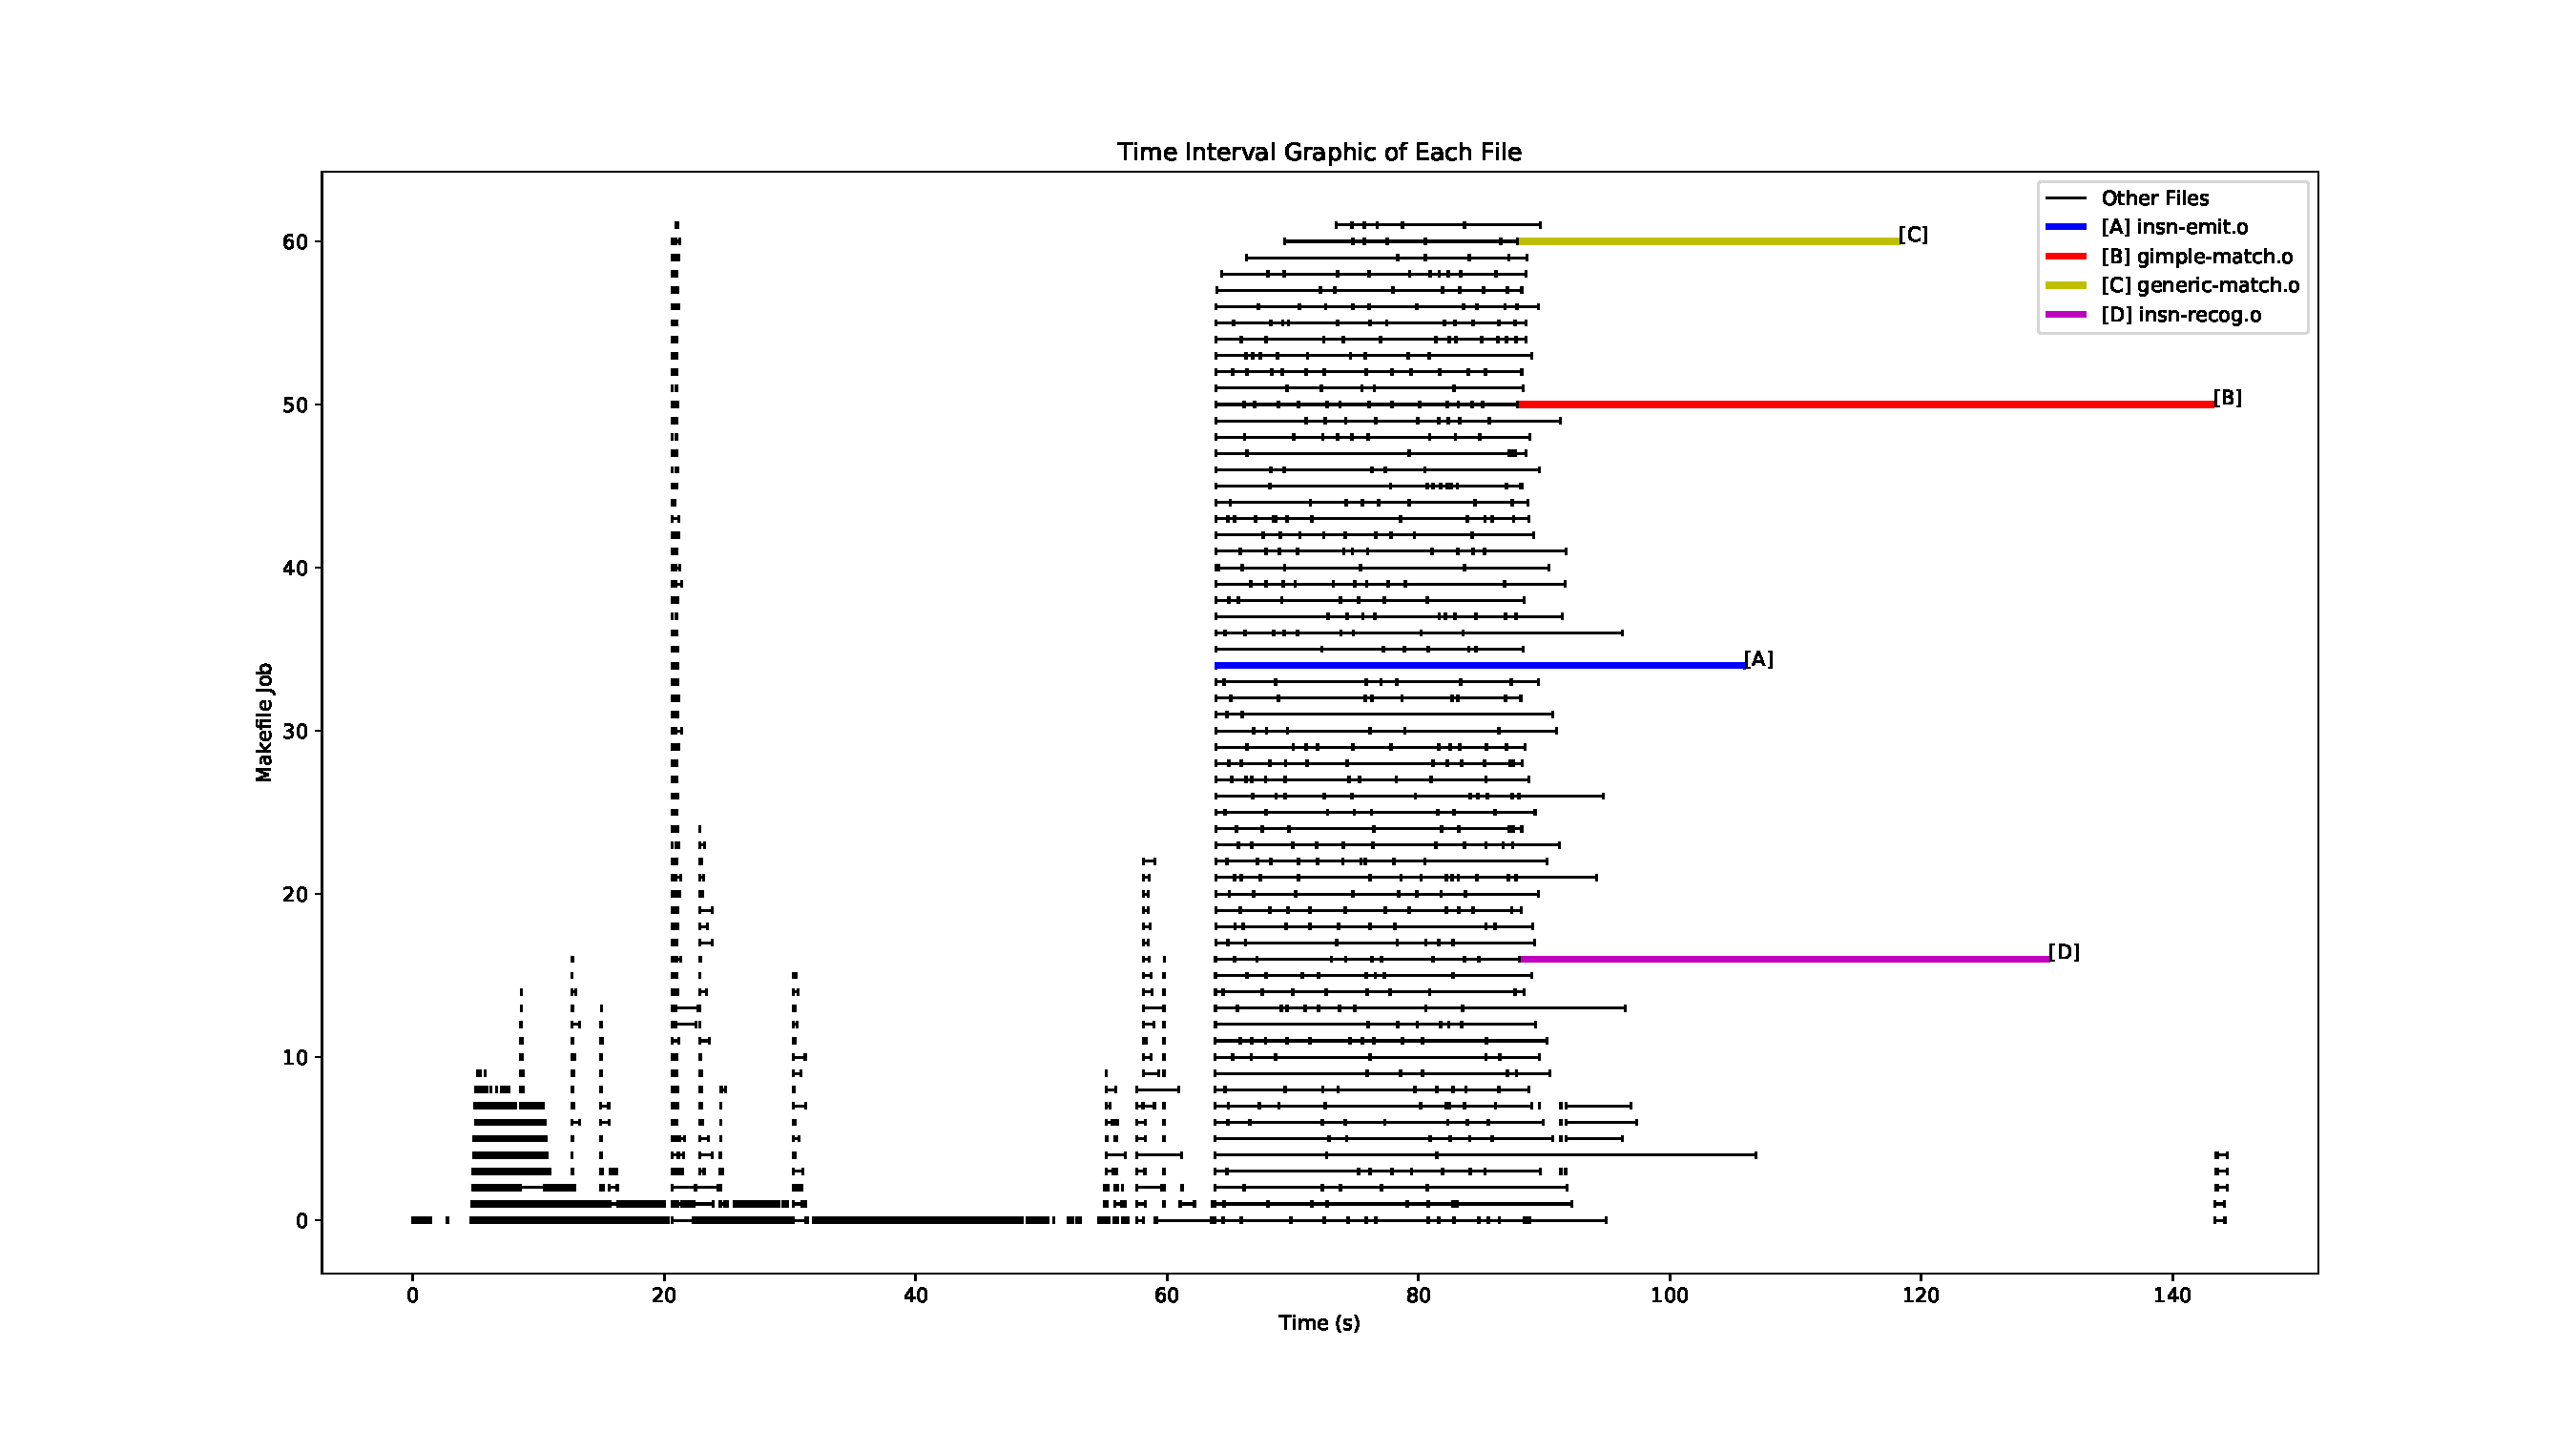
\includegraphics[scale=0.6, angle=-90]{gcc_timer_classic.pdf}
 \caption{Tempo corrido na compilação do GCC em um processador de 64 núcleos. Sem \textit{Bootstrap}}
 \label{fig:analysis_classical}
\end{figure}


%%%%%

\chapter{Conclusions}
\label{chap:conclusions}

We have presented two ways of parallelizing a compiler. Our first approach
involved parallelizing the application of intraprocedural optimizations in
parallel to each function, using threads. Although this predicted a $1.68\times$
speedup on GCC, its implementation showed to be difficult because of the heavy
use of global variables in the software.  We even got to a point where
analyzers such as helgrind and thread sanitizer were not detecting the race
conditions due to the race window being too small. Therefore, this approach may
not be adequate for already existing industrial-scale compilers for adding
parallelism.

However, if we are designing a compiler from the ground up, this approach may
be better from a software engineering perspective, as it becomes easier to add
multithreading to a part of the code that was, at least at some point, designed
with this in mind. We also get the advantage of avoiding the overheads
associated with process creation, such as page copying, etc.

Threading the compiler may also be the only option when parallelizing the
parser or interprocedural analysis, otherwise, there would be a huge amount of
interprocess communication. However, Figure \ref{fig:parallel_estimate} shows
that parsing is not a computer-intensive task. This is already parallel in LTO
by reading the multiple files, therefore this may not be of concern on present
days nor in the short future. However, the interprocess analysis is of concern,
once it is the only sequential step on LTO and may dominate the compilation
time on manycore machines just by being sequential.

On our second approach, we show how to use the already-existing LTO engine in
GCC to compile single files in parallel. The clear advantage of this approach
is how fast we got the first results when compared to threading the compiler,
and how fast we got it into a complete working condition (bootstrap the
compiler, testsuite acceptance, fuzzer testing).

Although the results were better than the threaded version ($1.88\times$ vs. $2.4\times$),
one may argue that the reason for that is due to our threaded implementation
not being as optimized as the LTO based version -- which is true -- and the
contrary must be expected because the cost of launching a thread is smaller
than the cost of launching a process plus all the necessary page copying.
Therefore, we may expect even larger speedups when compared to the LTO version
on optimized implementations.

From now on, we will focus on the LTO implementation results to drive our
conclusions. We archived up to $35\%$ speedup when comparing our results with
the \texttt{make -j64} alone, and no significant slowdown when compared to the
sequential version (even if there was, the developer could simply disable the
parallel compilation if this is observed). The reason for this is the existence
of files with large TU in the GCC project, as shown in Figure
\ref{fig:analysis_classical}, and this result might be interesting when the project
uses autogenerated (blob) C++ files. We also found a small speedup on Git,
which we find interesting because it consists of small files. One explanation
for this is that it does not have enough files to fully populate the manycore
machine's CPU.

As for the electrical energy usage, we show a reduction in power draw by the
CPU when compiling GCC with our options enabled. On Figure \ref{fig:power},
we observe a significant reduction in the peak power usage on the parallel
version. It may be that there is a point when the processor is in partial usage
(not in full usage) and may draw the same amount of power as if it is in full
usage. Therefore, for better energy efficiency, we should use the maximum power
of the CPU in the shortest amount of time to get a task done -- and this will
also save energy --.
%%%%%


%\providecommand\aviso[1]{
  \clearpage
  \null
  \vfill
  \begin{hyphenrules}{nohyphenation}
    \centering\bfseries\Large
    #1\par
  \end{hyphenrules}
  \vfill
  \clearpage
}

\providecommand\avisoFolhasDeRosto{
  \aviso{
    {\huge Você precisa editar os arquivos no diretório ``\texttt{conteudo}''!}
    \par\bigskip\bigskip\bigskip\bigskip
    Para gerar a capa e demais páginas preliminares no formato correto,
    modifique os arquivos ``\texttt{conteudo/paginas-preliminares.tex}'' e
    ``\texttt{conteudo/metadados.tex}'', usando como base os arquivos
    correspondentes no diretório ``\texttt{conteudo-exemplo}''.
  }
}

\providecommand\avisoCapitulos{
  \aviso{
    Insira o conteúdo dos capítulos do seu trabalho no arquivo
    ``\texttt{capitulos.tex}'' do diretório ``\texttt{conteudo}''.
  }
}

\providecommand\avisoApendices{
  \aviso{
    Insira o conteúdo dos apêndices do seu trabalho no arquivo
    ``\texttt{apendices.tex}'' do diretório ``\texttt{conteudo}''.
  }
}

\providecommand\avisoAnexos{
  \aviso{
    Insira o conteúdo dos anexos do seu trabalho no arquivo
    ``\texttt{anexos.tex}'' do diretório ``\texttt{conteudo}''.
  }
}

\providecommand\avisoArtigo{
  \aviso{
    Insira o conteúdo do artigo no arquivo ``\texttt{corpo-artigo.tex}''
    do diretório ``\texttt{conteudo}''. Não se esqueça de consultar
    o exemplo no diretório ``\texttt{conteudo-exemplo}'' para a
    definição do título, autoria etc.
  }
}

\providecommand\avisoApresentacao{
  \begin{frame}{Insira o conteúdo!}
  \aviso{
    Insira o conteúdo da apresentação no arquivo ``\texttt{corpo-apresentacao.tex}''
    do diretório ``\texttt{conteudo}''. Não se esqueça de consultar
    o exemplo no diretório ``\texttt{conteudo-exemplo}'' para a
    definição do título, autoria, estrutura etc.
  }
  \end{frame}
}

\providecommand\avisoPoster{
  \aviso{
    Insira o conteúdo do poster no arquivo ``\texttt{corpo-poster.tex}''
    do diretório ``\texttt{conteudo}''. Não se esqueça de consultar
    o exemplo no diretório ``\texttt{conteudo-exemplo}'' para a
    definição do título, autoria, estrutura etc.
  }
}

%\avisoCapitulos

% Os capítulos de compõem a dissertação/tese, com numeração normal, podem
% ser inseridos diretamente aqui ou "puxados" de outros arquivos.
% Em alguns (raros) casos, pode ser interessante usar \include ao
% invés de \input: https://tex.stackexchange.com/a/32058/183146

%\input{conteudo/01...}
%\par

%\input{conteudo/02...}
%\par
